% =============================================================================
%  raylib from Zero - a hands-on manual
%  Build with:  pdflatex raylib-manual.tex   (run it twice for the TOC)
% =============================================================================
\documentclass[11pt,a4paper,openany]{report}

\usepackage[T1]{fontenc}
\usepackage[utf8]{inputenc}
\usepackage[english]{babel}
\usepackage{lmodern}
\usepackage{microtype}
\usepackage[a4paper,top=2.4cm,bottom=2.4cm,left=2.6cm,right=2.6cm,headheight=22pt]{geometry}
\usepackage{amsmath}
\usepackage{xcolor}
\usepackage{graphicx}
\usepackage{listings}
\usepackage{mdframed}
\usepackage{titlesec}
\usepackage{enumitem}
\usepackage{booktabs}
\usepackage{fancyhdr}
\usepackage{tikz}
\usepackage{caption}
\usepackage[hidelinks]{hyperref}

\usetikzlibrary{arrows.meta,positioning,calc,shapes.geometric}

% ---- palette ---------------------------------------------------------------
\definecolor{rlink}{HTML}{1B6AC9}
\definecolor{rink}{HTML}{1F2430}
\definecolor{rgrey}{HTML}{6B7280}
\definecolor{rlight}{HTML}{F4F5F7}
\definecolor{rred}{HTML}{C0392B}
\definecolor{rgreen}{HTML}{2E7D32}
\definecolor{rblue}{HTML}{1565C0}
\definecolor{rorange}{HTML}{E07B00}
\definecolor{rpurple}{HTML}{6A3D9A}
\definecolor{codebg}{HTML}{F7F7F4}
\definecolor{codeframe}{HTML}{DDDDD6}
\definecolor{cmtcol}{HTML}{6C8A56}
\definecolor{kwcol}{HTML}{9C27B0}
\definecolor{strcol}{HTML}{B85C00}
\definecolor{numcol}{HTML}{B0B0A8}

\hypersetup{colorlinks=true,linkcolor=rlink,urlcolor=rlink,
            pdftitle={raylib from Zero},pdfauthor={}}

% ---- headings --------------------------------------------------------------
\titleformat{\chapter}[display]
  {\sffamily\bfseries}
  {\normalsize\color{rgrey}\MakeUppercase{\chaptertitlename}\ \thechapter}
  {6pt}
  {\color{rink}\Huge}
  [\vspace{2pt}{\color{rorange}\rule{\textwidth}{1.2pt}}]
\titlespacing*{\chapter}{0pt}{-14pt}{22pt}

\titleformat{\section}{\sffamily\large\bfseries\color{rink}}{\thesection}{0.7em}{}
\titleformat{\subsection}{\sffamily\normalsize\bfseries\color{rink}}{\thesubsection}{0.7em}{}
\titlespacing*{\section}{0pt}{16pt}{6pt}
\titlespacing*{\subsection}{0pt}{12pt}{4pt}

\setlength{\parindent}{0pt}
\setlength{\parskip}{6pt plus 2.5pt minus 1.5pt}
\widowpenalty=600
\clubpenalty=600
\raggedbottom

\pagestyle{fancy}
\fancyhf{}
\fancyhead[L]{\sffamily\footnotesize\color{rgrey}\leftmark}
\fancyhead[R]{\sffamily\footnotesize\color{rgrey}\thepage}
\renewcommand{\headrulewidth}{0.4pt}
\renewcommand{\headrule}{\hbox to\headwidth{\color{codeframe}\leaders\hrule height \headrulewidth\hfill}}
\renewcommand{\chaptermark}[1]{\markboth{\thechapter.\ #1}{}}

% ---- code ------------------------------------------------------------------
\lstdefinestyle{c}{
  language=C,
  basicstyle=\ttfamily\footnotesize,
  keywordstyle=\color{kwcol}\bfseries,
  commentstyle=\color{cmtcol}\itshape,
  stringstyle=\color{strcol},
  numberstyle=\ttfamily\tiny\color{numcol},
  backgroundcolor=\color{codebg},
  frame=single,
  rulecolor=\color{codeframe},
  framesep=7pt,
  xleftmargin=10pt,
  xrightmargin=2pt,
  breaklines=true,
  breakatwhitespace=true,
  showstringspaces=false,
  columns=fullflexible,
  keepspaces=true,
  tabsize=4,
  morekeywords={Vector2,Vector3,Color,Rectangle,Camera2D,Camera3D,Camera,
                BoundingBox,Texture2D,Texture,Image,Ray,RayCollision,Model,
                Font,bool,true,false,Sound,Music}
}
\lstset{style=c}

\lstdefinestyle{plain}{
  basicstyle=\ttfamily\footnotesize,
  backgroundcolor=\color{codebg},
  frame=single,
  rulecolor=\color{codeframe},
  framesep=7pt,
  xleftmargin=10pt,
  breaklines=true,
  keywordstyle={},
  commentstyle={},
  columns=fullflexible,
  keepspaces=true
}

% ---- callout boxes ---------------------------------------------------------
\newmdenv[
  linewidth=0pt,
  backgroundcolor=rlight,
  leftline=true,linecolor=rorange,linewidth=3pt,
  innerleftmargin=10pt,innerrightmargin=10pt,
  innertopmargin=8pt,innerbottommargin=8pt,
  skipabove=10pt,skipbelow=10pt,
  nobreak=true
]{gotchabox}

\newmdenv[
  linewidth=0pt,
  backgroundcolor=rlight,
  leftline=true,linecolor=rblue,linewidth=3pt,
  innerleftmargin=10pt,innerrightmargin=10pt,
  innertopmargin=8pt,innerbottommargin=8pt,
  skipabove=10pt,skipbelow=10pt,
  nobreak=true
]{keybox}

\newmdenv[
  linewidth=0pt,
  backgroundcolor=rlight,
  leftline=true,linecolor=rgreen,linewidth=3pt,
  innerleftmargin=10pt,innerrightmargin=10pt,
  innertopmargin=8pt,innerbottommargin=8pt,
  skipabove=10pt,skipbelow=10pt,
  nobreak=true
]{trybox}

\newcommand{\boxtitle}[2]{{\sffamily\bfseries\small\color{#1}#2}\par\vspace{2pt}}
\newcommand{\gotcha}[1]{\begin{gotchabox}\boxtitle{rorange}{WATCH OUT}#1\end{gotchabox}}
\newcommand{\keyidea}[1]{\begin{keybox}\boxtitle{rblue}{THE KEY IDEA}#1\end{keybox}}
\newcommand{\tryit}[2]{\begin{trybox}\boxtitle{rgreen}{RUN IT}#1\par\vspace{3pt}{\ttfamily\small #2}\end{trybox}}

\newcommand{\file}[1]{{\ttfamily\small #1}}

% =============================================================================
\begin{document}

% ---- title page ------------------------------------------------------------
\begin{titlepage}
\centering
\vspace*{2.2cm}

{\sffamily\bfseries\fontsize{46}{52}\selectfont\color{rink} raylib\par}
\vspace{4pt}
{\sffamily\fontsize{46}{52}\selectfont\color{rorange} from Zero\par}

\vspace{1.0cm}
{\color{rorange}\rule{0.62\textwidth}{1.4pt}\par}
\vspace{0.9cm}

{\sffamily\Large\color{rink} A hands-on manual for someone who has\\[3pt]
never drawn a single triangle in 3D\par}

\vspace{1.6cm}

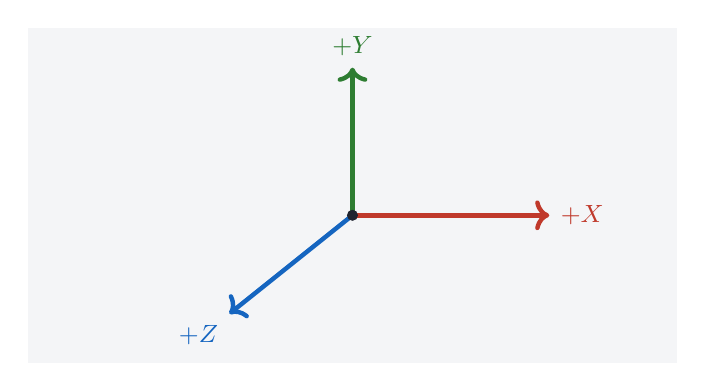
\begin{tikzpicture}[scale=1.25]
  \fill[rlight] (-3.3,-1.5) rectangle (3.3,1.9);
  \draw[->,rred,line width=1.6pt]   (0,0) -- (2.0,0)      node[right] {\sffamily\small $+X$};
  \draw[->,rgreen,line width=1.6pt] (0,0) -- (0,1.5)      node[above] {\sffamily\small $+Y$};
  \draw[->,rblue,line width=1.6pt]  (0,0) -- (-1.25,-1.0) node[below left] {\sffamily\small $+Z$};
  \fill[rink] (0,0) circle (1.6pt);
\end{tikzpicture}

\vspace{1.6cm}

{\sffamily\color{rgrey}\large Window and frame loop $\cdot$ drawing $\cdot$ input $\cdot$ cameras\\[3pt]
2D and 3D $\cdot$ collisions $\cdot$ and a silly little Doom at the end\par}

\vfill
{\sffamily\small\color{rgrey} Written against raylib 6.1-dev \quad$\cdot$\quad all code in this manual compiles and runs\par}
\end{titlepage}

\tableofcontents
\thispagestyle{empty}
\clearpage
\setcounter{page}{1}

\part{Making a game}

\chapter{Before we start}

\section{What raylib actually is}

raylib is a C library that hands you a window, a keyboard, a mouse, a sound card
and a way to put coloured pixels on screen. That is it. It is not an engine.
There is no editor, no scene graph, no entity system, no asset pipeline, no
project format. You write a \lstinline|main()|, you call some functions, you get
a game.

That is the reason it feels strange at first if you are used to tools that hand
you a scene and ask you to fill it in. In raylib \emph{you} own the loop. Nothing
happens that you did not write a line for.

The whole library is about 500 functions, and they are named so plainly that you
can usually guess them: \lstinline|DrawCircle|, \lstinline|IsKeyDown|,
\lstinline|LoadTexture|, \lstinline|CheckCollisionRecs|. There is no official
reference manual, on purpose --- the header file \file{raylib.h} \emph{is} the
documentation, one line of comment per function, and the examples are the
tutorial.

\keyidea{If you remember one thing from this manual, remember this: the
\file{raylib.h} header is the documentation. Open it. Search it. Every function
you will ever use is in there with a one-line comment explaining it.}

\section{What you need to know already}

C. Not advanced C --- variables, \lstinline|if|, \lstinline|while|, functions,
arrays and structs are enough. Every piece of code in this manual stays inside
that. You do not need pointers-to-pointers, you do not need
\lstinline|malloc|, and you certainly do not need C++.

You do \emph{not} need any 3D background. Chapters 9 to 14 assume you have never
seen a 3D coordinate system in your life, and build it up from a single arrow on
a page.

\section{The files that come with this manual}

This manual is not a thing to read in an armchair. Every chapter has a matching
program you can run, change and break. They live in two folders next to it:

\begin{center}
\begin{tabular}{@{}lll@{}}
\toprule
\textbf{Folder} & \textbf{Part} & \textbf{What is in it} \\
\midrule
\file{course2d/} & I & the fundamentals: window, loop, shapes, input, collisions, camera \\
\file{course3d/} & I & the 3D half: axes, cameras, movement, collisions, the mini Doom \\
\file{cheatsheet/} & II & one example per module of the official raylib cheatsheet \\
\bottomrule
\end{tabular}
\end{center}

Each folder has a \file{build.sh} that compiles and runs one of them:

\begin{lstlisting}[style=plain]
./course2d/build.sh 1        # builds and runs course2d/lesson01_window.c
./course3d/build.sh 7        # builds and runs the mini Doom
./cheatsheet/build.sh 9      # builds and runs the audio module example
\end{lstlisting}

Part I is a path: read it in order and you end up with a game. Part II is a
reference: each chapter stands alone, so read the one you need when you need it.

The script needs the raylib library to have been built once. If you have never
run the project, do that first from the root folder:

\begin{lstlisting}[style=plain]
make                         # builds bin/Debug/libraylib.a and the sample app
\end{lstlisting}

\section{What a build actually needs}

When people get stuck on day one, it is almost never the code --- it is the
compiler command. There is no magic in it, so here it is in full, the one that
\file{build.sh} runs for you:

\begin{lstlisting}[style=plain]
cc  mygame.c                                   # your source file
    -o mygame                                  # the program to produce
    -I build/external/raylib-master/src        # where raylib.h lives
    bin/Debug/libraylib.a                      # the library itself
    -lpthread -lm -ldl -lrt -lX11              # what raylib needs on Linux
\end{lstlisting}

Three ingredients, always: your \file{.c} file, the \emph{header} so the compiler
knows the function signatures, and the \emph{library} so the linker can find the
actual code. If you get \lstinline|raylib.h: No such file| you got the
\lstinline|-I| wrong. If you get \lstinline|undefined reference to InitWindow|
you got the library path wrong. Those two errors mean two very different things
and mixing them up costs beginners hours.

\gotcha{The order matters on Linux: the library goes \emph{after} your
\file{.c} file on the command line, never before. GNU \lstinline|ld| resolves
symbols left to right, and a library listed first has nothing left to resolve.}

\section{How to read this manual}

Read a chapter, then run its lesson, then go back and change three numbers in the
lesson until something breaks. That third step is the one that actually teaches
you. Nothing here can be damaged: the worst that happens is a black window, and
you press Escape.

The boxes mean:

\gotcha{A mistake almost everyone makes here. Reading these will save you an
afternoon each.}

\keyidea{The one sentence from the section that is worth carrying with you.}

\tryit{The lesson that shows this chapter running.}{./course2d/build.sh 1}

\chapter{The shape of every raylib program}

\section{Immediate mode, and why nothing stays on screen}

Here is the idea that everything else in raylib hangs from. Most graphical
toolkits you have met are \emph{retained mode}: you create a button object, you
add it to a window, and it stays there. The toolkit remembers it and redraws it
for you.

raylib is \emph{immediate mode}. Nothing is remembered. There is no circle
object. \lstinline|DrawCircle()| does not create a circle --- it paints circle
shaped pixels, right now, and then forgets all about it. If you want the circle
to still be there in a sixtieth of a second, you call \lstinline|DrawCircle()|
again.

\keyidea{Your program repaints the entire picture, from a blank canvas,
sixty times a second. Everything you can see on screen is something you drew
this frame. Everything you stop drawing disappears instantly.}

This sounds wasteful and it is not: GPUs are extremely good at exactly this. And
it buys you something precious for a beginner --- there is no hidden state. If
something is on screen, a line in your code put it there this frame. If something
is missing, a line in your code did not run. Debugging graphics becomes reading
your own draw calls in order.

\section{The skeleton}

Every raylib program, from the ten line example to the full game, has this shape:

\begin{lstlisting}
#include "raylib.h"

int main(void)
{
    InitWindow(800, 450, "My game");   // 1. once: open the window
    SetTargetFPS(60);

    while (!WindowShouldClose())       // 2. the frame loop
    {
        // UPDATE: change variables, draw nothing

        BeginDrawing();                // 3. start painting
            ClearBackground(RAYWHITE);
            DrawText("Hello", 20, 20, 20, DARKGRAY);
        EndDrawing();                  // 4. show it
    }

    CloseWindow();                     // 5. once: clean up
    return 0;
}
\end{lstlisting}

That is lesson 1 of the 2D course, near enough. Let us take the five parts apart.

\begin{center}
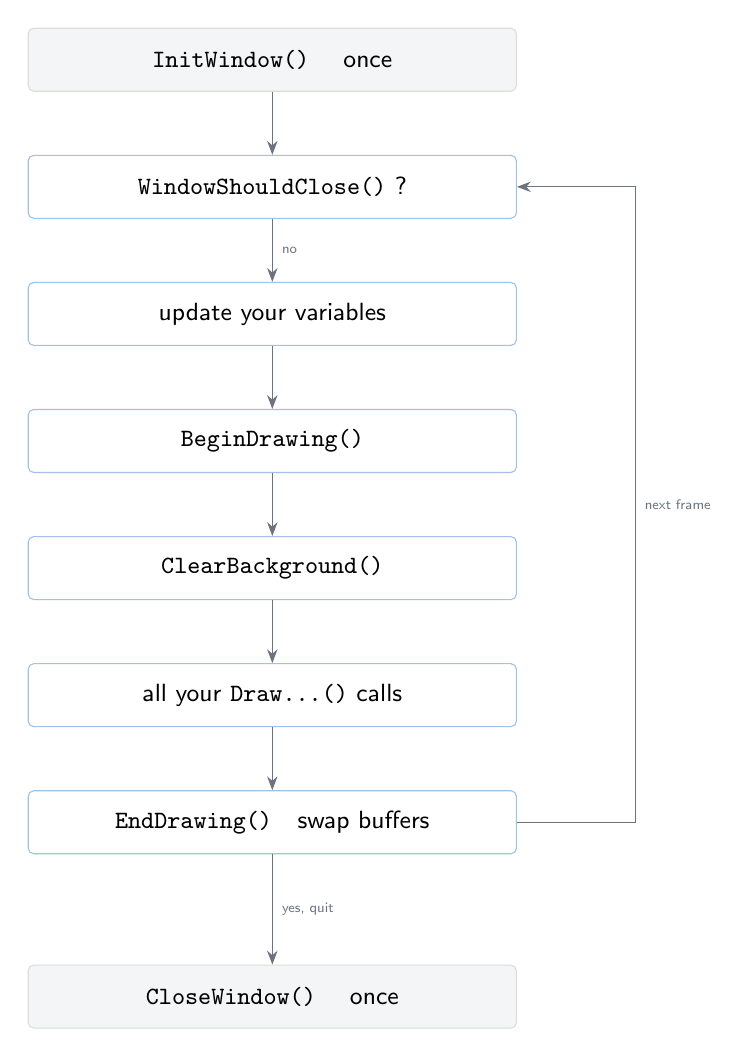
\begin{tikzpicture}[
  node distance=8mm,
  every node/.style={font=\sffamily\small},
  bx/.style={draw=codeframe,fill=rlight,rounded corners=2pt,minimum width=6.2cm,minimum height=8mm,align=center},
  lbx/.style={bx,fill=white,draw=rblue!40},
  arrow/.style={-{Stealth[length=5pt]},rgrey}
]
\node[bx] (init) {\texttt{InitWindow()} \quad once};
\node[lbx,below=of init] (check) {\texttt{WindowShouldClose()} ?};
\node[lbx,below=of check] (update) {update your variables};
\node[lbx,below=of update] (begin) {\texttt{BeginDrawing()}};
\node[lbx,below=of begin] (clear) {\texttt{ClearBackground()}};
\node[lbx,below=of clear] (draw) {all your \texttt{Draw...()} calls};
\node[lbx,below=of draw] (end) {\texttt{EndDrawing()} \ \ swap buffers};
\node[bx,below=14mm of end] (close) {\texttt{CloseWindow()} \quad once};

\draw[arrow] (init) -- (check);
\draw[arrow] (check) -- node[right,font=\sffamily\tiny,text=rgrey] {no} (update);
\draw[arrow] (update) -- (begin);
\draw[arrow] (begin) -- (clear);
\draw[arrow] (clear) -- (draw);
\draw[arrow] (draw) -- (end);
\draw[arrow] (end.east) -- ++(1.5,0) |- node[right,pos=0.25,font=\sffamily\tiny,text=rgrey] {next frame} (check.east);
\draw[arrow] (end) -- node[right,font=\sffamily\tiny,text=rgrey] {yes, quit} (close);
\end{tikzpicture}
\end{center}

\subsection{1. InitWindow}

\lstinline|InitWindow(width, height, title)| creates the window and, more
importantly, the OpenGL context behind it. Until this line runs, no other raylib
function works --- not loading a texture, not measuring text, nothing. Calling
\lstinline|LoadTexture()| before \lstinline|InitWindow()| is a classic
first-day crash.

Flags are the exception: \lstinline|SetConfigFlags()| must be called
\emph{before} \lstinline|InitWindow()|, because it configures how the window
gets created. The two you will want:

\begin{lstlisting}
SetConfigFlags(FLAG_VSYNC_HINT | FLAG_MSAA_4X_HINT);
InitWindow(800, 450, "My game");
\end{lstlisting}

\lstinline|FLAG_VSYNC_HINT| syncs your drawing to the monitor's refresh so the
image does not tear. \lstinline|FLAG_MSAA_4X_HINT| turns on antialiasing so
diagonal edges stop looking like staircases.

\subsection{2. WindowShouldClose}

\lstinline|while (!WindowShouldClose())| is your game loop. The function returns
true when the user presses Escape or clicks the window's close button, so the
loop reads as ``keep going until they want out''.

Each pass through this loop is one \emph{frame}. At 60 FPS the body of that loop
runs 60 times a second, which gives you about 16 milliseconds to do everything.

\subsection{3 and 4. BeginDrawing and EndDrawing}

This pair is where the confusion usually is, so let us be precise.

\lstinline|BeginDrawing()| says ``I am about to paint''. It prepares the canvas
for this frame. Every \lstinline|Draw...()| call after it adds geometry to a
batch that raylib is accumulating.

\lstinline|EndDrawing()| does three jobs at once:

\begin{enumerate}[leftmargin=*,itemsep=2pt]
  \item it flushes the batch --- everything you queued actually gets sent to the
        GPU and drawn;
  \item it swaps the buffers. You have been painting on a hidden canvas the whole
        time; this is the moment it becomes the visible one. That is
        \emph{double buffering}, and it is why you never see a half-drawn frame;
  \item it polls input events and waits, if needed, to hit your target frame rate.
\end{enumerate}

\gotcha{Nothing appears on screen until \lstinline|EndDrawing()| runs. If you
put a \lstinline|sleep()| or a long loop between \lstinline|BeginDrawing()| and
\lstinline|EndDrawing()| hoping to see an animation, you will see nothing at all
but a frozen window. Animation happens \emph{across} frames, never inside one.}

\subsection{ClearBackground}

The window still holds last frame's pixels. \lstinline|ClearBackground(RAYWHITE)|
wipes them. Skip it and you get smears --- which, incidentally, is a fun thing to
try once on purpose: comment it out in lesson 1 and move something around.

\section{Update and draw: keep them apart}

Notice how the skeleton has a comment saying ``UPDATE'' before
\lstinline|BeginDrawing()|. That separation is not enforced by raylib, it is a
discipline, and it is worth adopting from day one:

\begin{itemize}[leftmargin=*,itemsep=2pt]
  \item \textbf{Update} --- read input, move things, run the AI, check
        collisions. Change variables. Draw nothing.
  \item \textbf{Draw} --- paint the current state of those variables. Change nothing.
\end{itemize}

When the two get tangled you end up with bugs where an object reacts to a
collision that was resolved half a frame ago, and they are miserable to find.
Keeping them apart costs nothing and every lesson in this course does it.

\section{Frame rate, and the two ways to control it}

\lstinline|SetTargetFPS(60)| tells raylib to throttle the loop to at most 60
iterations per second. Without it your loop runs as fast as the machine allows,
burning 100\% of a CPU core to draw frames nobody will see.

\lstinline|FLAG_VSYNC_HINT| does a similar job at a different level: it makes the
buffer swap wait for the monitor. In practice, set both; they cooperate.

Two useful readings, both free:

\begin{lstlisting}
int   fps = GetFPS();          // frames per second, as an integer
float dt  = GetFrameTime();    // seconds the LAST frame took: ~0.0166 at 60fps
double t  = GetTime();         // seconds since InitWindow()
\end{lstlisting}

\lstinline|GetFrameTime()| is the important one and it gets its own chapter
(chapter 5). It is the difference between a game that behaves the same on every
computer and one that does not.

\tryit{Lesson 1 prints the frame counter, the elapsed time and the frame
duration, live. Watch the frame counter climb and realise that every one of those
numbers was repainted from scratch.}{./course2d/build.sh 1}

\chapter{The screen: coordinates, colour, shapes}

\section{Where is (0,0)?}

Top left corner. X grows to the right, Y grows \emph{downwards}.

\begin{center}
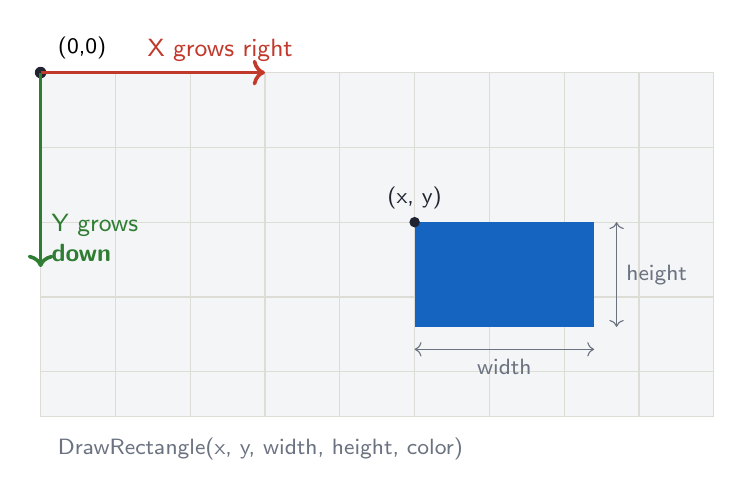
\begin{tikzpicture}[scale=0.95,every node/.style={font=\sffamily\small}]
  \fill[rlight] (0,0) rectangle (9,-4.6);
  \draw[codeframe] (0,0) rectangle (9,-4.6);
  \foreach \x in {1,2,...,8} \draw[codeframe] (\x,0) -- (\x,-4.6);
  \foreach \y in {1,2,3,4} \draw[codeframe] (0,-\y) -- (9,-\y);

  \fill[rink] (0,0) circle (2.2pt);
  \node[above right,font=\sffamily\footnotesize] at (0.1,0.05) {(0,0)};

  \draw[->,rred,line width=1.3pt] (0,0) -- (3,0) node[above,pos=0.8] {X grows right};
  \draw[->,rgreen,line width=1.3pt] (0,0) -- (0,-2.6) node[right,pos=0.85,align=left] {Y grows\\ \textbf{down}};

  \fill[rblue] (5,-2) rectangle (7.4,-3.4);
  \fill[rink] (5,-2) circle (2pt);
  \node[above,font=\sffamily\footnotesize,text=rink] at (5,-1.95) {(x, y)};
  \draw[<->,rgrey] (5,-3.7) -- node[below,font=\sffamily\footnotesize] {width} (7.4,-3.7);
  \draw[<->,rgrey] (7.7,-2) -- node[right,font=\sffamily\footnotesize] {height} (7.7,-3.4);

  \node[below right,font=\sffamily\footnotesize,text=rgrey] at (0.1,-4.75) {DrawRectangle(x, y, width, height, color)};
\end{tikzpicture}
\end{center}

If you did maths at school, Y pointing down feels wrong. It comes from how
screens were scanned, line by line from the top, and every 2D graphics API on
earth inherited it.

\gotcha{In 3D (chapter 9) Y goes back to pointing \emph{up}. Same letter,
opposite direction, in the same program, sometimes on the same screen. When
something moves the wrong way vertically, this is the first thing to check:
which of the two worlds am I in?}

Two helpers give you the current window size, and you should prefer them over
hardcoding the numbers you passed to \lstinline|InitWindow|, because the window
can be resized:

\begin{lstlisting}
int w = GetScreenWidth();
int h = GetScreenHeight();
DrawText("centred-ish", w/2 - 60, h/2, 20, DARKGRAY);
\end{lstlisting}

\section{Corners and centres}

\lstinline|DrawRectangle| takes the \textbf{top-left corner}.
\lstinline|DrawCircle| takes the \textbf{centre}. That inconsistency has burned
every raylib beginner, so hold on to it:

\begin{lstlisting}
DrawRectangle(100, 100, 80, 40, MAROON);   // corner at (100,100), 80x40
DrawCircle(100, 100, 30, DARKBLUE);        // CENTRE at (100,100), radius 30
\end{lstlisting}

If you want a rectangle centred at a point, you subtract half its size yourself:

\begin{lstlisting}
DrawRectangle(cx - w/2, cy - h/2, w, h, MAROON);
\end{lstlisting}

You will write that line a thousand times. In the 3D chapters it comes back as
\lstinline|BoxFromCenter()|, which is the same idea with one more axis.

\section{Rectangle, the struct you will live in}

\begin{lstlisting}
typedef struct Rectangle {
    float x;        // LEFT edge
    float y;        // TOP edge
    float width;
    float height;
} Rectangle;
\end{lstlisting}

Many functions take one of these instead of four loose numbers, and the
collision functions all do. Get used to building them inline:

\begin{lstlisting}
Rectangle player = { 100, 100, 40, 40 };
DrawRectangleRec(player, DARKBLUE);
DrawRectangleLinesEx(player, 2, BLACK);
\end{lstlisting}

\section{Colour}

A \lstinline|Color| is four bytes, each 0 to 255:

\begin{lstlisting}
typedef struct Color { unsigned char r, g, b, a; } Color;

Color myOrange = { 230, 120, 20, 255 };          // opaque
Color ghost    = { 230, 120, 20, 90 };           // mostly transparent
\end{lstlisting}

\lstinline|a| is alpha: 255 is solid, 0 is invisible. raylib ships about
twenty-five named colours --- \lstinline|RAYWHITE|, \lstinline|DARKGRAY|,
\lstinline|MAROON|, \lstinline|SKYBLUE|, \lstinline|GOLD|, \lstinline|BLANK|
(fully transparent) and friends --- and one very handy helper:

\begin{lstlisting}
DrawRectangle(10, 10, 100, 100, Fade(BLUE, 0.5f));   // BLUE at 50% alpha
\end{lstlisting}

\lstinline|Fade| returns a copy of the colour with the alpha scaled. Use it for
shadows, overlays, ghosts and dimmed HUDs instead of writing the struct out.

\gotcha{When you write a colour inline you need the cast, because C needs to
know what the braces mean: \lstinline|DrawRectangle(0,0,10,10,(Color){20,20,25,255})|.
Forgetting the \lstinline|(Color)| gives you a confusing compiler error about
initialisation.}

\section{The order of your draw calls is the layer order}

There is no z-index, no layer system and no sorting. Whatever you draw last is
on top. Painting a picture, literally.

\begin{lstlisting}
DrawRectangle(640, 340, 100, 100, DARKPURPLE);   // painted first: underneath
DrawCircle(700, 400, 45, GOLD);                  // painted last:  on top
\end{lstlisting}

That means the structure of your draw section is your scene's depth. Background
first, then the world, then characters, then effects, then the HUD last of all.
When something is mysteriously invisible, nine times out of ten it is being drawn
\emph{before} something opaque.

\section{Text}

\begin{lstlisting}
DrawText("Hello", 20, 20, 20, DARKGRAY);        // text, x, y, fontSize, color
int width = MeasureText("Hello", 20);           // how wide would it be?
\end{lstlisting}

\lstinline|MeasureText| is how you centre text, since there is no alignment
parameter:

\begin{lstlisting}
const char *txt = "GAME OVER";
DrawText(txt, GetScreenWidth()/2 - MeasureText(txt, 60)/2, 200, 60, RED);
\end{lstlisting}

And to print variables, \lstinline|TextFormat| is raylib's
\lstinline|sprintf| that manages the buffer for you:

\begin{lstlisting}
DrawText(TextFormat("score: %i   time: %.2f", score, GetTime()), 20, 20, 20, BLACK);
\end{lstlisting}

\gotcha{\lstinline|TextFormat| writes into an internal rotating buffer. It is
perfect for drawing this frame and wrong for storing: never keep the returned
pointer across frames, copy the string if you need it later.}

\section{The shapes you actually use}

There are about forty drawing functions; these are the ones that cover almost
everything:

\begin{center}
\begin{tabular}{@{}ll@{}}
\toprule
\textbf{Function} & \textbf{Notes} \\
\midrule
\lstinline|DrawRectangle(x,y,w,h,c)| & corner based \\
\lstinline|DrawRectangleRec(rec,c)| & takes a \lstinline|Rectangle| \\
\lstinline|DrawRectangleLinesEx(rec,thick,c)| & outline with thickness \\
\lstinline|DrawRectangleRounded(rec,round,seg,c)| & rounded corners \\
\lstinline|DrawCircle(cx,cy,r,c)| & centre based \\
\lstinline|DrawCircleLines(cx,cy,r,c)| & outline \\
\lstinline|DrawLine(x1,y1,x2,y2,c)| & one pixel thin \\
\lstinline|DrawLineEx(v1,v2,thick,c)| & with thickness \\
\lstinline|DrawTriangle(v1,v2,v3,c)| & \textbf{counter-clockwise} vertices \\
\lstinline|DrawPoly(centre,sides,r,rot,c)| & regular polygon \\
\bottomrule
\end{tabular}
\end{center}

The naming pattern repeats across the whole library and is worth learning as a
rule rather than as forty separate facts:

\begin{itemize}[leftmargin=*,itemsep=2pt]
  \item plain name, e.g. \lstinline|DrawCircle| --- the simple version, loose
        \lstinline|int| coordinates;
  \item \textbf{V} suffix, e.g. \lstinline|DrawCircleV| --- same thing but taking
        a \lstinline|Vector2|;
  \item \textbf{Rec} suffix --- takes a \lstinline|Rectangle|;
  \item \textbf{Ex} suffix --- extended: extra parameters like thickness;
  \item \textbf{Pro} suffix --- all the knobs: origin, rotation, scaling;
  \item \textbf{Lines} in the name --- outline instead of filled.
\end{itemize}

Once you see that, you can guess most of raylib without looking anything up.

\gotcha{\lstinline|DrawTriangle| wants its three vertices in counter-clockwise
order. Give them clockwise and the triangle is facing away from you, so it gets
culled and you see nothing at all. If a triangle is invisible, swap two of its
vertices before you look for any other bug.}

\tryit{Lesson 2 draws the coordinate grid, every basic shape labelled, alpha
blending, and lets you swap the draw order with SPACE to watch the layering
change.}{./course2d/build.sh 2}

\chapter{Input}

\section{Three questions you can ask about a key}

This is short but it matters enormously, because picking the wrong one of the
three is the most common beginner bug in any engine.

\begin{center}
\begin{tabular}{@{}lll@{}}
\toprule
\textbf{Function} & \textbf{True when} & \textbf{Use it for} \\
\midrule
\lstinline|IsKeyDown(KEY_D)| & every frame it is held & walking, aiming, holding \\
\lstinline|IsKeyPressed(KEY_D)| & the single frame it goes down & jump, shoot, menus \\
\lstinline|IsKeyReleased(KEY_D)| & the single frame it comes up & charge-and-release \\
\bottomrule
\end{tabular}
\end{center}

Hold a key for one second at 60 FPS: \lstinline|IsKeyDown| is true sixty times,
\lstinline|IsKeyPressed| is true once.

\gotcha{Use \lstinline|IsKeyDown| for a menu and your cursor jumps sixty entries
in one second. Use \lstinline|IsKeyPressed| for walking and your character
teleports one step per tap and refuses to walk. When input ``feels broken'',
check which of the two you used before anything else.}

Key names are the obvious ones: \lstinline|KEY_A| to \lstinline|KEY_Z|,
\lstinline|KEY_ZERO| to \lstinline|KEY_NINE|, \lstinline|KEY_SPACE|,
\lstinline|KEY_ENTER|, \lstinline|KEY_LEFT_SHIFT|, \lstinline|KEY_LEFT_CONTROL|,
\lstinline|KEY_UP|, \lstinline|KEY_LEFT|, \lstinline|KEY_TAB|,
\lstinline|KEY_ESCAPE|. They are all listed in \file{raylib.h} under
\lstinline|KeyboardKey|.

\gotcha{\lstinline|KEY_ESCAPE| closes the window by default --- that is what
\lstinline|WindowShouldClose()| watches. If you want Escape to open a pause menu
instead, turn the default off with \lstinline|SetExitKey(KEY_NULL)| and handle it
yourself.}

\section{The mouse}

\begin{lstlisting}
Vector2 mouse = GetMousePosition();      // in SCREEN pixels
float   wheel = GetMouseWheelMove();     // -1, 0 or +1 sized steps
Vector2 delta = GetMouseDelta();         // how far it moved THIS frame

if (IsMouseButtonPressed(MOUSE_BUTTON_LEFT))  { /* click */ }
if (IsMouseButtonDown(MOUSE_BUTTON_RIGHT))    { /* held */ }
\end{lstlisting}

The same pressed/down/released trio applies to buttons.

\lstinline|GetMouseDelta()| is the one that makes first person cameras possible.
It reports movement rather than position, which is exactly what you want when
the cursor is locked in place and can no longer move:

\begin{lstlisting}
DisableCursor();     // hide the cursor and lock it to the window centre
EnableCursor();      // give it back to the user
\end{lstlisting}

With the cursor disabled, \lstinline|GetMousePosition()| stops being useful
(the pointer is pinned) but \lstinline|GetMouseDelta()| keeps reporting how much
the user moved the physical mouse. Chapter 12 turns that into a camera.

\gotcha{Always call \lstinline|EnableCursor()| before \lstinline|CloseWindow()|,
or a crash can leave the user's pointer captured and invisible. Every lesson in
the 3D course does this.}

\section{Text input}

For a name entry field you do not want key codes, you want characters, with the
keyboard layout and the shift key already applied:

\begin{lstlisting}
int c = GetCharPressed();
while (c > 0)
{
    if ((c >= 32) && (c <= 125) && (length < MAX)) name[length++] = (char)c;
    c = GetCharPressed();   // the queue may hold several this frame
}
if (IsKeyPressed(KEY_BACKSPACE) && length > 0) name[--length] = '\0';
\end{lstlisting}

It is a queue, so you loop until it is empty. Handle backspace with
\lstinline|IsKeyPressed| because it is an action, not a character.

\tryit{Lesson 3 shows the pressed-versus-down counters side by side. Hold SPACE
for a second and compare the two numbers.}{./course2d/build.sh 3}

\chapter{Time, and why everything is multiplied by delta time}

\section{The problem}

Here is a piece of code that looks completely reasonable and is wrong:

\begin{lstlisting}
if (IsKeyDown(KEY_D)) player.x += 5;      // WRONG
\end{lstlisting}

It says ``move five pixels per frame''. On a 60 Hz monitor that is 300 pixels a
second. On a 144 Hz monitor it is 720. On a machine struggling at 30 FPS it is
150. Your game is a different game on every computer, and if the frame rate
stutters, the physics stutter with it.

\section{The fix}

\lstinline|GetFrameTime()| returns how long the previous frame took, in seconds.
People universally call it \emph{delta time}, or \lstinline|dt|. At 60 FPS it is
about \lstinline|0.0166|; at 120 FPS about \lstinline|0.0083|.

\begin{lstlisting}
float dt = GetFrameTime();
float speed = 300.0f;                         // PIXELS PER SECOND

if (IsKeyDown(KEY_D)) player.x += speed*dt;   // RIGHT
\end{lstlisting}

At 60 FPS that adds $300 \times 0.0166 = 5$ pixels. At 120 FPS it adds
$300 \times 0.0083 = 2.5$ pixels, twice as often. Same distance per second, on
every machine.

\keyidea{Every speed you write down is per \emph{second}, and every time you
apply it you multiply by \lstinline|dt|. Not sometimes --- always. Movement,
rotation, timers, fading, reloading, animation. If a number changes over time,
it is multiplied by \lstinline|dt|.}

\section{Reading a movement line}

Once the habit sticks, your constants start documenting themselves:

\begin{lstlisting}
float walkSpeed = 4.0f;       // metres per second  -> a person walking
float runSpeed  = 8.0f;       // metres per second  -> a person running
float turnSpeed = 90.0f;      // degrees per second -> a quarter turn each second
float reload    = 1.5f;       // seconds
\end{lstlisting}

Compare that with ``0.066 per frame'' and you can see which version you would
rather debug at midnight.

\section{Timers}

The same logic drives anything that happens after a delay. Add \lstinline|dt| to
a counter and check it:

\begin{lstlisting}
float shootCooldown = 0.0f;

// update
if (shootCooldown > 0.0f) shootCooldown -= dt;

if (IsMouseButtonPressed(MOUSE_BUTTON_LEFT) && shootCooldown <= 0.0f)
{
    Shoot();
    shootCooldown = 0.25f;     // four shots per second, on any machine
}
\end{lstlisting}

Animation is the same pattern, and lesson 5 uses exactly this shape to step
through a sprite sheet.

\gotcha{Do not use \lstinline|GetTime()| for this. \lstinline|GetTime()| is
absolute seconds since startup: fine for a clock, awkward for ``0.25 seconds from
now'' because you have to remember when now was. Counting down a float with
\lstinline|dt| is simpler and pauses for free when you stop updating it.}

\section{The one case where delta time bites back}

If the game freezes for a second --- a big file loads, you dragged the window,
you hit a breakpoint --- the next \lstinline|dt| is huge. Everything moves a
second's worth in one frame, and fast objects teleport straight through walls,
because the collision check only looks at where they \emph{landed}, not the path
they took.

The standard defence is one line, and it is why you often see this in real games:

\begin{lstlisting}
float dt = GetFrameTime();
if (dt > 0.05f) dt = 0.05f;    // never simulate more than 50 ms in one step
\end{lstlisting}

The game slows down briefly instead of exploding. Good enough for everything you
will write for a long while.

\tryit{Lesson 3 puts a green square that uses \lstinline|dt| next to a red square
that does not, and drives both from the same keys.}{./course2d/build.sh 3}

\chapter{Collisions in 2D: the rehearsal}

Everything in this chapter comes back, almost unchanged, in 3D. Learn it here
where you can see it, and chapter 13 will feel like a rerun.

\section{Detecting}

Two rectangles overlap if they overlap on \textbf{both} axes at once. One axis
where they do not overlap is enough to guarantee they are apart:

\begin{center}
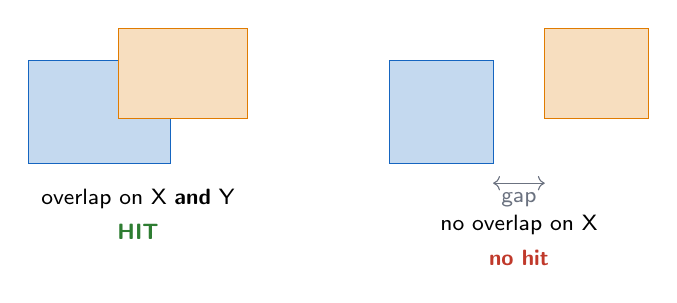
\begin{tikzpicture}[scale=0.82,every node/.style={font=\sffamily\footnotesize}]
  % case 1: overlap
  \begin{scope}
    \fill[rblue!25,draw=rblue] (0,0) rectangle (2.2,1.6);
    \fill[rorange!25,draw=rorange] (1.4,0.7) rectangle (3.4,2.1);
    \node at (1.7,-0.55) {overlap on X \textbf{and} Y};
    \node[text=rgreen] at (1.7,-1.05) {\textbf{HIT}};
  \end{scope}
  % case 2: no overlap on X
  \begin{scope}[xshift=5.6cm]
    \fill[rblue!25,draw=rblue] (0,0) rectangle (1.6,1.6);
    \fill[rorange!25,draw=rorange] (2.4,0.7) rectangle (4.0,2.1);
    \draw[<->,rgrey] (1.6,-0.3) -- node[below] {gap} (2.4,-0.3);
    \node at (2.0,-0.95) {no overlap on X};
    \node[text=rred] at (2.0,-1.45) {\textbf{no hit}};
  \end{scope}
\end{tikzpicture}
\end{center}

\begin{lstlisting}
bool overlapX = (a.x < b.x + b.width)  && (a.x + a.width  > b.x);
bool overlapY = (a.y < b.y + b.height) && (a.y + a.height > b.y);
bool hit = overlapX && overlapY;
\end{lstlisting}

raylib gives you that in one call, and a few relatives:

\begin{lstlisting}
CheckCollisionRecs(recA, recB);                        // box vs box
CheckCollisionCircles(centreA, rA, centreB, rB);       // circle vs circle
CheckCollisionCircleRec(centre, radius, rec);          // circle vs box
CheckCollisionPointRec(GetMousePosition(), button);    // is the mouse over it?
\end{lstlisting}

That last one is how you write a button without any UI library: a
\lstinline|Rectangle|, a \lstinline|CheckCollisionPointRec|, and
\lstinline|IsMouseButtonPressed|. Three lines, and you own it completely.

\section{Resolving, which is the hard half}

Knowing that you hit a wall does not stop you. The naive fix --- ``if I hit
something, do not move at all'' --- produces a game that feels awful: walk into a
wall at a slight angle and you stop dead instead of sliding along it.

The trick is to treat the axes separately:

\begin{center}
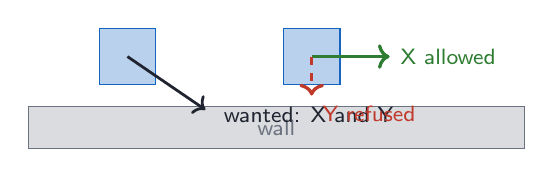
\begin{tikzpicture}[scale=0.9,every node/.style={font=\sffamily\footnotesize}]
  \fill[rgrey!25,draw=rgrey] (0,0) rectangle (7,0.6);
  \node[text=rgrey] at (3.5,0.3) {wall};

  \fill[rblue!30,draw=rblue] (1,0.9) rectangle (1.8,1.7);
  \draw[->,rink,line width=1pt] (1.4,1.3) -- (2.5,0.55) node[right,pos=1.1] {wanted: X and Y};

  \fill[rblue!30,draw=rblue] (3.6,0.9) rectangle (4.4,1.7);
  \draw[->,rgreen,line width=1.2pt] (4.0,1.3) -- (5.1,1.3) node[right] {X allowed};
  \draw[->,rred,line width=1.2pt,dashed] (4.0,1.3) -- (4.0,0.75) node[below right] {Y refused};
\end{tikzpicture}
\end{center}

\begin{lstlisting}
// 1. try the X move on its own
Rectangle attempt = player;
attempt.x += dx;
if (!HitsAnyWall(attempt)) player.x = attempt.x;   // otherwise: keep old x

// 2. try the Y move on its own
attempt = player;
attempt.y += dy;
if (!HitsAnyWall(attempt)) player.y = attempt.y;   // otherwise: keep old y
\end{lstlisting}

Walking diagonally into a horizontal wall, the Y step is refused and the X step
is allowed, so you slide along it. That is the whole secret, and it is the same
code in 3D with \lstinline|z| in place of \lstinline|y|.

\keyidea{Detect with one call. Resolve one axis at a time. Two moves, two
checks, never both at once.}

\section{Keeping things on screen}

The cheapest collision of all, and one every game needs:

\begin{lstlisting}
if (player.x < 0) player.x = 0;
if (player.y < 0) player.y = 0;
if (player.x + player.width  > GetScreenWidth())  player.x = GetScreenWidth()  - player.width;
if (player.y + player.height > GetScreenHeight()) player.y = GetScreenHeight() - player.height;
\end{lstlisting}

Note it clamps \emph{after} the move rather than refusing it. For a wall you want
to refuse the move; for a screen edge, clamping feels better because the player
keeps sliding along the border.

\tryit{Lesson 4 has a little maze. SPACE switches the walls between ``solid''
(resolved per axis) and ``ghost'' (detected only) so you can feel the
difference.}{./course2d/build.sh 4}

\chapter{Images, textures and sprites}

\section{Two things that sound identical and are not}

\begin{center}
\begin{tabular}{@{}lll@{}}
\toprule
 & \textbf{\lstinline|Image|} & \textbf{\lstinline|Texture2D|} \\
\midrule
Lives in & normal RAM (CPU) & video memory (GPU) \\
You can  & read and edit pixels & draw it, fast \\
You cannot & draw it & edit single pixels \\
Typical use & load, resize, recolour & everything you see \\
\bottomrule
\end{tabular}
\end{center}

The usual flow is: get an \lstinline|Image|, upload it once, throw the
\lstinline|Image| away, draw the \lstinline|Texture2D| forever.

\begin{lstlisting}
Image img = LoadImage("player.png");        // into RAM
ImageResize(&img, 64, 64);                  // cheap to edit here
Texture2D tex = LoadTextureFromImage(img);  // upload to the GPU
UnloadImage(img);                           // the RAM copy is dead weight now
\end{lstlisting}

If you do not need to touch the pixels, \lstinline|LoadTexture("player.png")|
does all four steps for you.

\section{The golden rule of loading}

\gotcha{Load \textbf{outside} the loop, unload \textbf{after} the loop. Calling
\lstinline|LoadTexture()| inside the frame loop uploads a fresh copy to the GPU
sixty times a second. A minute later you are out of video memory and you have no
idea why.}

\begin{lstlisting}
Texture2D tex = LoadTexture("player.png");   // once

while (!WindowShouldClose())
{
    BeginDrawing();
        DrawTexture(tex, 100, 100, WHITE);   // every frame: just draws
    EndDrawing();
}

UnloadTexture(tex);                          // once
CloseWindow();
\end{lstlisting}

The same rule covers fonts, sounds, music and models. Every
\lstinline|Load...| has a matching \lstinline|Unload...|, and they belong on
either side of the loop.

\section{Drawing a texture, four ways}

\begin{lstlisting}
DrawTexture(tex, x, y, WHITE);                       // plain, at a position
DrawTextureV(tex, position, WHITE);                  // same, Vector2
DrawTextureEx(tex, position, rotation, scale, WHITE);// rotated and scaled
DrawTextureRec(tex, source, position, WHITE);        // just a PIECE of it
DrawTexturePro(tex, source, dest, origin, rot, WHITE); // everything at once
\end{lstlisting}

That \lstinline|WHITE| at the end is the \emph{tint}: the texture's colours get
multiplied by it. \lstinline|WHITE| means ``unchanged''. Pass \lstinline|RED| and
everything goes red; pass \lstinline|Fade(WHITE, 0.5f)| and the sprite is half
transparent. This is how you flash a character on damage without a second image.

\section{Sprite sheets}

An animation is not many files, it is one image holding many frames side by side,
plus a \lstinline|Rectangle| that says which frame to show:

\begin{center}
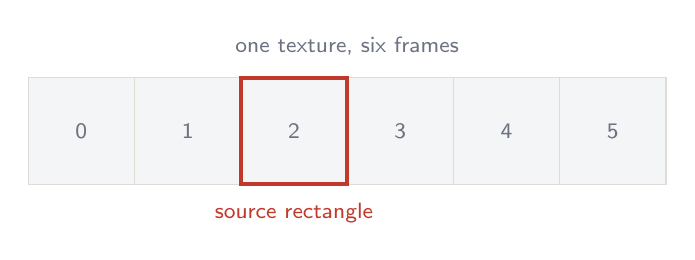
\begin{tikzpicture}[scale=0.9,every node/.style={font=\sffamily\footnotesize}]
  \foreach \i in {0,1,2,3,4,5} {
    \draw[codeframe,fill=rlight] (\i*1.5,0) rectangle (\i*1.5+1.5,1.5);
    \node[text=rgrey] at (\i*1.5+0.75,0.75) {\i};
  }
  \draw[rred,line width=1.4pt] (3,0) rectangle (4.5,1.5);
  \node[text=rred] at (3.75,-0.4) {source rectangle};
  \node[text=rgrey] at (4.5,1.95) {one texture, six frames};
\end{tikzpicture}
\end{center}

\begin{lstlisting}
Rectangle source = { frame*FRAME_SIZE, 0, FRAME_SIZE, FRAME_SIZE };
DrawTextureRec(sheet, source, position, WHITE);
\end{lstlisting}

And you advance \lstinline|frame| on a timer, never on a frame counter, for the
reason chapter 5 gave:

\begin{lstlisting}
frameTimer += dt;
while (frameTimer >= frameDuration)
{
    frameTimer -= frameDuration;
    frame = (frame + 1) % FRAME_COUNT;
}
\end{lstlisting}

\gotcha{To flip a sprite horizontally, make the source rectangle's
\lstinline|width| \emph{negative}. It reads like a bug and it is the intended
API: \lstinline|source.width *= -1| and your character faces the other way,
with no second image and no rotation.}

\section{Where files are looked for}

Paths are relative to the \emph{working directory}, which is wherever you
launched the program from, not where the executable sits. That is why running
from an IDE sometimes finds your \file{.png} and running from a terminal does
not.

This project ships a helper for exactly that, in \file{src/resource\_dir.h}:

\begin{lstlisting}
SearchAndSetResourceDir("resources");   // find it and chdir there
Texture2D tex = LoadTexture("wabbit_alpha.png");
\end{lstlisting}

\gotcha{A texture that failed to load is not a crash: you get a texture with
\lstinline|id == 0| and you draw nothing, silently. If a sprite is invisible,
check \lstinline|IsTextureValid(tex)| before suspecting your draw code.}

\tryit{Lesson 5 builds a six frame sprite sheet in memory --- no external files
--- and plays it back, showing the whole sheet, the current frame, and the source
rectangle moving across it.}{./course2d/build.sh 5}

\chapter{Camera2D: world coordinates and the Begin/End idea}

\section{The problem with drawing in pixels}

Everything so far has been drawn at screen pixels. That works until the world is
bigger than the window. Then you find yourself writing
\lstinline|DrawRectangle(enemy.x - scrollX, enemy.y - scrollY, ...)| on every
single draw call, and forgetting the subtraction on one of them.

The fix is to stop thinking in pixels. Store everything in \textbf{world}
coordinates --- metres, tiles, whatever your game is made of --- and let a camera
decide which part of the world the window is looking at.

\section{Camera2D}

\begin{lstlisting}
typedef struct Camera2D {
    Vector2 offset;     // where the target lands ON SCREEN (usually the middle)
    Vector2 target;     // the WORLD point the camera is centred on
    float rotation;     // degrees; rotates the whole world
    float zoom;         // 1.0 normal, 2.0 twice as big. Never 0.
} Camera2D;
\end{lstlisting}

The pair that confuses people is \lstinline|target| and \lstinline|offset|. Read
it as a sentence: \emph{``the world point \lstinline|target| is displayed at the
screen position \lstinline|offset|''}. So to centre the camera on the player you
set \lstinline|target| to the player's world position and \lstinline|offset| to
the middle of the window:

\begin{lstlisting}
camera.target = player;                                         // world
camera.offset = (Vector2){ GetScreenWidth()/2.0f, GetScreenHeight()/2.0f };
camera.zoom   = 1.0f;
\end{lstlisting}

\gotcha{\lstinline|zoom| defaults to \lstinline|0| if you write
\lstinline|Camera2D camera = { 0 }| and forget to set it --- and a zoom of zero
scales the entire world down to nothing. Black screen, no error, no clue. If your
Camera2D shows nothing, this is why, every time.}

\section{The Begin/End pair, which is the real lesson}

\begin{lstlisting}
BeginMode2D(camera);
    // WORLD coordinates in here. The camera transforms everything.
    DrawRectangle(player.x, player.y, 30, 30, BLUE);
EndMode2D();

// SCREEN pixels again out here. Nothing below moves with the camera.
DrawText("HEALTH 100", 20, 20, 20, RAYWHITE);
\end{lstlisting}

\keyidea{Inside \lstinline|BeginMode2D|/\lstinline|EndMode2D| you are in world
space and the camera moves things around. Outside, you are in screen pixels and
nothing moves. The HUD goes outside. Always.}

This is worth dwelling on, because in three chapters' time you will meet
\lstinline|BeginMode3D| / \lstinline|EndMode3D| and it is the same idea with a
different camera: the \lstinline|Begin| pushes a transform, the \lstinline|End|
pops it. Your health bar sits outside the pair in both cases, for exactly the
same reason.

You can even nest them in one frame: draw the world in 3D, end the 3D mode, draw
a 2D minimap and the HUD. That is precisely what the mini Doom in chapter 14
does.

\section{Going between the two worlds}

Sooner or later you need to know what the mouse is pointing at in world
coordinates --- to click an enemy, to place a tile:

\begin{lstlisting}
Vector2 worldPoint  = GetScreenToWorld2D(GetMousePosition(), camera);
Vector2 screenPoint = GetWorldToScreen2D(enemy.position, camera);
\end{lstlisting}

The second one is how you put a floating name tag above a character: compute
where the character is on screen, then draw text there \emph{outside} the
Begin/End pair so it keeps a constant size no matter the zoom. The 3D course
uses the 3D version of this same function to label the axes in lesson 1.

\section{Making the camera feel good}

A camera nailed to the player is correct and slightly nauseating. Real games lag
behind a little. One line, using \lstinline|dt| as always:

\begin{lstlisting}
camera.target.x += (player.x - camera.target.x)*5.0f*dt;
camera.target.y += (player.y - camera.target.y)*5.0f*dt;
\end{lstlisting}

Each frame the camera closes a fraction of the gap towards the player. Larger
number, tighter follow. This is called exponential smoothing and it is worth
knowing because it makes almost anything feel better: camera follow, aiming,
health bars catching up to the real value.

\tryit{Lesson 6 gives you a world far bigger than the window, with zoom and
rotation, and a red crosshair drawn \emph{outside} the Begin/End pair so you can
watch it refuse to move with the world.}{./course2d/build.sh 6}

\chapter{Into 3D: the three axes}

\section{One new number}

A 3D point is a 2D point with a third number bolted on. That is genuinely all
that changes at the level of data:

\begin{lstlisting}
typedef struct Vector2 { float x, y; } Vector2;
typedef struct Vector3 { float x, y, z; } Vector3;
\end{lstlisting}

What changes is what those numbers \emph{mean}, and that is where the
disorientation comes from, so let us be very clear about it.

\section{Which way each axis points}

\begin{center}
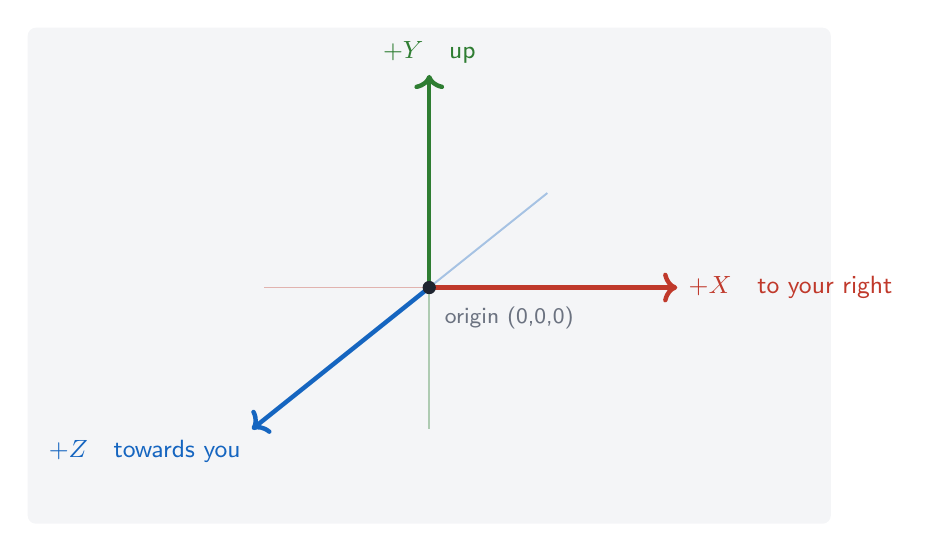
\begin{tikzpicture}[scale=1.5,every node/.style={font=\sffamily\small}]
  \fill[rlight,rounded corners=3pt] (-3.4,-2.0) rectangle (3.4,2.2);

  \draw[->,rred,line width=1.6pt]   (0,0) -- (2.1,0)       node[right]      {$+X$ \ \ to your right};
  \draw[->,rgreen,line width=1.6pt] (0,0) -- (0,1.8)       node[above]      {$+Y$ \ \ up};
  \draw[->,rblue,line width=1.6pt]  (0,0) -- (-1.5,-1.2)   node[below left] {$+Z$ \ \ towards you};

  \draw[rred,line width=0.7pt,opacity=0.35]   (0,0) -- (-1.4,0);
  \draw[rgreen,line width=0.7pt,opacity=0.35] (0,0) -- (0,-1.2);
  \draw[rblue,line width=0.7pt,opacity=0.35]  (0,0) -- (1.0,0.8);

  \fill[rink] (0,0) circle (1.6pt);
  \node[below right,font=\sffamily\footnotesize,text=rgrey] at (0.05,-0.08) {origin (0,0,0)};
\end{tikzpicture}
\end{center}

\begin{center}
\begin{tabular}{@{}llll@{}}
\toprule
\textbf{Axis} & \textbf{Negative} & \textbf{Positive} & \textbf{Think of it as} \\
\midrule
X & left & right & sideways \\
Y & down & \textbf{up} & \textbf{height} \\
Z & far away & towards you & depth \\
\bottomrule
\end{tabular}
\end{center}

This is a \emph{right-handed} system, the same as OpenGL. If you want to check it
physically: point your right thumb along $+X$ and your index finger along $+Y$,
and your middle finger points along $+Z$, out of the screen at you.

\gotcha{Y now points \textbf{up}. In the 2D half of this manual it pointed
\textbf{down}. Both are true, in their own space, and both are live in the same
program --- a 3D game with a HUD uses both in the same frame. When something
moves vertically the wrong way, ask yourself which space that line is in.}

\section{The floor is the XZ plane}

This is the sentence that makes 3D click for most people.

Height is Y. So a floor --- a flat surface at a constant height --- is all the
points where Y is the same, usually zero. The two axes left over, X and Z, are
the ones you walk around on.

\begin{itemize}[leftmargin=*,itemsep=2pt]
  \item A top-down map of your level only needs X and Z. That is why the minimap
        in chapter 14 maps world X to screen X and world Z to screen Y.
  \item \lstinline|DrawGrid(20, 1.0f)| draws its grid on the XZ plane at
        $Y = 0$, because that is the floor.
  \item Walking means changing X and Z. Jumping means changing Y.
\end{itemize}

\keyidea{X and Z are the ground. Y is how high you are. A character walking
around a room is a 2D problem in X and Z, with a Y that mostly stays at one
value.}

\section{Objects sit on the floor, they do not live at zero}

\lstinline|DrawCube| takes the \textbf{centre} of the cube. So a cube of height 2
resting on the floor has its centre at $Y = 1$, not $Y = 0$. Put it at zero and
half the cube is buried underground.

\begin{lstlisting}
DrawCube((Vector3){ 0, 1, 0 }, 2, 2, 2, MAROON);   // a 2x2x2 cube ON the floor
\end{lstlisting}

And mind the parameter order, which quietly encodes the axes:

\begin{lstlisting}
DrawCube(centre, width, height, length, colour);
//               ^X     ^Y      ^Z
\end{lstlisting}

\lstinline|width| is the size along X, \lstinline|height| along Y,
\lstinline|length| along Z. There is a \lstinline|DrawCubeV| that takes a
\lstinline|Vector3| size instead, which removes the ambiguity, and it is the one
worth preferring once the axes are second nature.

\section{Units}

raylib has no opinion about what one unit means. Pick one and keep it. This
course uses \textbf{one unit = one metre}, so every number you write is something
you can picture:

\begin{lstlisting}
#define EYE_HEIGHT  1.7f    // a person's eyes
float walkSpeed =   4.0f;   // metres per second, a brisk walk
\end{lstlisting}

Once your constants are in metres and seconds, you can spot a wrong number just
by reading it.

\tryit{Lesson 1 of the 3D course draws the three axes in their standard colours
--- X red, Y green, Z blue --- and lets you jump the camera onto each axis in
turn with the keys 1 to 4.}{./course3d/build.sh 1}

\chapter{The 3D camera}

\section{It is five numbers, and none of them are magic}

\begin{lstlisting}
typedef struct Camera3D {
    Vector3 position;     // where the eye is
    Vector3 target;       // the world point it is looking at
    Vector3 up;           // which way is "up" for the camera
    float fovy;           // vertical field of view, in DEGREES
    int projection;       // CAMERA_PERSPECTIVE or CAMERA_ORTHOGRAPHIC
} Camera3D;
\end{lstlisting}

\begin{center}
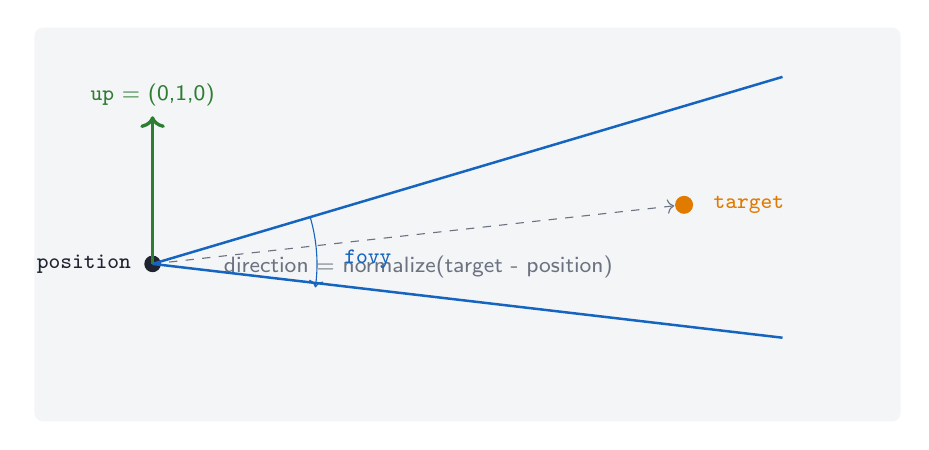
\begin{tikzpicture}[scale=1.25,every node/.style={font=\sffamily\footnotesize}]
  \fill[rlight,rounded corners=3pt] (-1.2,-1.6) rectangle (7.6,2.4);

  % eye
  \fill[rink] (0,0) circle (2.4pt);
  \node[left,text=rink] at (-0.12,0) {\texttt{position}};

  % target
  \fill[rorange] (5.4,0.6) circle (2.6pt);
  \node[right,text=rorange] at (5.6,0.6) {\texttt{target}};

  % view direction
  \draw[->,rgrey,dashed] (0,0) -- (5.3,0.59);
  \node[below,text=rgrey] at (2.7,0.18) {direction = normalize(target - position)};

  % frustum
  \draw[rblue,line width=0.9pt] (0,0) -- (6.4,1.9);
  \draw[rblue,line width=0.9pt] (0,0) -- (6.4,-0.75);
  \draw[rblue,->] (1.6,0.48) arc (16.5:-8:1.7);
  \node[right,text=rblue] at (1.85,0.05) {\texttt{fovy}};

  % up
  \draw[->,rgreen,line width=1.2pt] (0,0) -- (0,1.5);
  \node[above,text=rgreen] at (0,1.5) {\texttt{up} = (0,1,0)};
\end{tikzpicture}
\end{center}

Notice what is \emph{not} in that struct: there is no field for the direction the
camera is facing, and no rotation angles. The direction is worked out from the
two points:

\[ \text{direction} = \text{normalize}(\text{target} - \text{position}) \]

Which gives you the two operations you will use forever:

\begin{itemize}[leftmargin=*,itemsep=2pt]
  \item \textbf{To turn the camera}: move the \lstinline|target|, leave
        \lstinline|position| alone.
  \item \textbf{To move the camera}: move \lstinline|position| \emph{and}
        \lstinline|target| by the same amount, so it does not turn while it
        travels.
\end{itemize}

\gotcha{Move only \lstinline|position| and the camera swings round to keep
staring at the old target, like a security camera tracking you. That is
occasionally what you want and usually a bug.}

\section{fovy, or choosing a lens}

\lstinline|fovy| is the vertical angle the camera can see, in degrees. It behaves
exactly like a camera lens:

\begin{center}
\begin{tabular}{@{}ll@{}}
\toprule
\textbf{fovy} & \textbf{Feels like} \\
\midrule
20--30 & telephoto: flat, compressed, distant \\
45 & neutral, good for inspecting an object \\
60--75 & the normal first person game range \\
90+ & fisheye: fast, dizzying, very wide \\
\bottomrule
\end{tabular}
\end{center}

Doom-like shooters tend to sit around 70 to 90, which is why the mini Doom in
chapter 14 uses 75.

\section{Perspective versus orthographic}

\lstinline|CAMERA_PERSPECTIVE| is what your eyes do: distant things look smaller,
parallel lines converge.

\lstinline|CAMERA_ORTHOGRAPHIC| removes that. Distance stops affecting size and
parallel lines stay parallel. This is the look of isometric strategy games, of
CAD, and of 2D games faking depth.

\gotcha{When you switch to orthographic, \lstinline|fovy| stops meaning degrees
and starts meaning \emph{how many world units fit vertically on screen}. Leave it
at 45 and your world is 45 metres tall in the window --- everything is a speck.
Set something like 10 and it looks sane again.}

\section{Begin and End, again}

\begin{lstlisting}
BeginMode3D(camera);
    DrawGrid(20, 1.0f);
    DrawCube((Vector3){ 0, 1, 0 }, 2, 2, 2, MAROON);
EndMode3D();

// back to 2D screen pixels: the HUD
DrawText("HEALTH 100", 20, 20, 20, RAYWHITE);
DrawFPS(10, 10);
\end{lstlisting}

Exactly the same contract as \lstinline|BeginMode2D| in chapter 8: inside is
world space, outside is screen pixels. Your crosshair, health bar, ammo counter
and minimap all go outside, and that is why they stay nailed to the window while
the world moves.

There is one extra thing \lstinline|BeginMode3D| does that the 2D version does
not: it enables the \textbf{depth buffer}. In 2D the draw order decided what was
on top; in 3D the GPU compares distances per pixel, so a cube behind another cube
is hidden correctly no matter which order you drew them in. You get that for
free.

\gotcha{Transparency is the exception. The depth buffer works per pixel, and a
half transparent surface writes depth as if it were solid, which can hide things
behind it. If you draw transparent objects, draw them after the opaque ones,
furthest first. You will not hit this for a while, but when a glass wall makes
things vanish, this is why.}

\section{The ready-made cameras}

Before writing your own, try raylib's:

\begin{lstlisting}
UpdateCamera(&camera, CAMERA_FREE);           // fly around: WASD, mouse, wheel
UpdateCamera(&camera, CAMERA_ORBITAL);        // spins around the target by itself
UpdateCamera(&camera, CAMERA_FIRST_PERSON);   // classic FPS
UpdateCamera(&camera, CAMERA_THIRD_PERSON);   // follows the target from behind
\end{lstlisting}

One line, in the update section, and the camera works. For first and third
person, call \lstinline|DisableCursor()| first so the mouse is captured.

They are perfect for looking at a model or prototyping a scene, and they run out
of road the moment you want collisions, crouching, recoil, a vehicle, or a camera
that does anything specific to your game. That is the subject of the next
chapter.

\tryit{Lesson 2 of the 3D course lets you move each of the five camera fields
with the keyboard and watch the numbers; lesson 3 cycles the four built-in modes
with TAB.}{./course3d/build.sh 2 \quad and \quad ./course3d/build.sh 3}

\chapter{Drawing 3D objects}

\section{The shapes that come in the box}

raylib has no 3D modelling tools, but it has enough primitives to build a whole
game out of, and every one of them is a single call:

\begin{lstlisting}
DrawCube(centre, width, height, length, colour);     // sizes are X, Y, Z
DrawCubeV(centre, size, colour);                     // same, size as Vector3
DrawCubeWires(centre, w, h, l, colour);              // just the edges
DrawSphere(centre, radius, colour);
DrawCylinder(bottomCentre, radiusTop, radiusBottom, height, sides, colour);
DrawPlane(centre, size2D, colour);                   // a flat XZ quad
DrawLine3D(from, to, colour);
DrawGrid(slices, spacing);                           // the XZ floor grid
\end{lstlisting}

A few things worth knowing before you use them:

\begin{itemize}[leftmargin=*,itemsep=3pt]
  \item \lstinline|DrawCube| takes the \textbf{centre}, like
        \lstinline|DrawCircle| did in 2D and unlike \lstinline|DrawRectangle|.
  \item \lstinline|DrawCylinder| takes the \textbf{bottom} centre, not the middle.
        Give it a top radius of 0 and you have a cone.
  \item \lstinline|DrawPlane| is always flat on the XZ plane. It takes a
        \lstinline|Vector2| size because a flat thing only has two dimensions.
  \item \lstinline|DrawGrid| is centred on the origin, so a grid over a level
        that starts at 0 and grows positive will only cover a quarter of it.
\end{itemize}

\section{Why everything looks flat}

The first 3D scene anybody draws looks like coloured paper cut-outs. Every face
of the cube is exactly the same shade, so the shape reads as a hexagon rather
than a box.

That is not a bug. Plain \lstinline|DrawCube| does no lighting at all --- there
is no light in the scene, so every surface just gets its flat colour. Real
lighting means shaders, which is a much later chapter of your life.

Three cheap tricks get you 90\% of the way, and the lessons use all three:

\begin{enumerate}[leftmargin=*,itemsep=3pt]
  \item \textbf{Draw the wireframe on top.} A cube plus its dark edges reads as a
        solid object immediately:
\begin{lstlisting}
DrawCube(p, 2, 2, 2, MAROON);
DrawCubeWires(p, 2, 2, 2, (Color){ 30, 26, 24, 255 });
\end{lstlisting}

  \item \textbf{Vary the colour per object.} Identical walls merge into one mass;
        a little variation separates them. The mini Doom shades each wall cell
        from its grid coordinates:
\begin{lstlisting}
int shade = 88 + ((col*7 + row*13) % 26);
\end{lstlisting}

  \item \textbf{Make the floor and ceiling different.} Two
        \lstinline|DrawPlane| calls in different colours do more for the sense of
        being inside a room than any amount of geometry.
\end{enumerate}

\section{A fake shadow}

Nothing tells you where an object is in 3D like a shadow, and a convincing one
costs one line: a very flat dark cube on the floor, directly under the object.

\begin{lstlisting}
DrawCube((Vector3){ obj.x, 0.01f, obj.z }, 1.0f, 0.02f, 1.0f, Fade(BLACK, 0.5f));
\end{lstlisting}

The \lstinline|0.01f| lifts it a hair above the floor. Put it at exactly
\lstinline|0| and it fights with the floor plane for the same pixels, which
produces a horrible flickering called \emph{z-fighting}. Whenever two surfaces
occupy the same plane and shimmer, nudge one of them.

\section{Making something face the player}

Enemies in early first person games were flat images that always turned to face
you. raylib does that with billboards:

\begin{lstlisting}
DrawBillboard(camera, texture, position, size, WHITE);
\end{lstlisting}

If you have no texture, you can still get the effect with geometry. Work out the
direction from the object to the camera, and place details along it --- this is
the trick the mini Doom uses to give its enemies eyes that follow you:

\begin{lstlisting}
Vector3 toPlayer = Vector3Normalize(Vector3Subtract(camera.position, e->position));
Vector3 side = Vector3Normalize(Vector3CrossProduct(toPlayer, (Vector3){ 0, 1, 0 }));
Vector3 base = Vector3Add(e->position, Vector3Scale(toPlayer, 0.22f));
DrawSphere(Vector3Add(base, Vector3Scale(side,  0.10f)), 0.055f, YELLOW);
DrawSphere(Vector3Add(base, Vector3Scale(side, -0.10f)), 0.055f, YELLOW);
\end{lstlisting}

That is the first time we have used the cross product for something practical.
Chapter 12 explains it properly; for now, read it as ``give me the direction
perpendicular to these two''.

\section{Models, when you outgrow cubes}

\begin{lstlisting}
Model model = LoadModel("robot.glb");        // once, outside the loop
DrawModel(model, position, scale, WHITE);    // every frame
DrawModelEx(model, position, rotAxis, rotAngle, scaleV, WHITE);
UnloadModel(model);                          // once, after the loop
\end{lstlisting}

Same load-outside-unload-after rule as textures. raylib reads \file{.obj},
\file{.gltf}, \file{.glb}, \file{.iqm} and \file{.vox}, and \file{.glb} is the
one to prefer because it packs the mesh, the materials and the textures into a
single file.

\section{The maths helpers}

Vector maths lives in a separate header you have to include yourself:

\begin{lstlisting}
#include "raymath.h"
\end{lstlisting}

The handful you will actually use:

\begin{center}
\begin{tabular}{@{}ll@{}}
\toprule
\textbf{Function} & \textbf{What it gives you} \\
\midrule
\lstinline|Vector3Add(a, b)| & a + b \\
\lstinline|Vector3Subtract(a, b)| & a $-$ b: the vector from b to a \\
\lstinline|Vector3Scale(v, f)| & v stretched by f \\
\lstinline|Vector3Length(v)| & how long it is \\
\lstinline|Vector3Normalize(v)| & same direction, length exactly 1 \\
\lstinline|Vector3Distance(a, b)| & distance between two points \\
\lstinline|Vector3CrossProduct(a, b)| & a direction perpendicular to both \\
\bottomrule
\end{tabular}
\end{center}

\keyidea{\lstinline|Vector3Normalize| is the one to understand. A normalized
vector has length 1, so it carries a \emph{direction} and nothing else. Multiply
it by a speed and you get a velocity; multiply it by a distance and you get an
offset. Almost every movement line in the next chapters is
\lstinline|normalize(something) * speed * dt|.}

\chapter{Your own first person camera}

This is the chapter people brace themselves for, and it is smaller than it looks.
There are two angles and one formula, and then you are done.

\section{The two angles}

\begin{center}
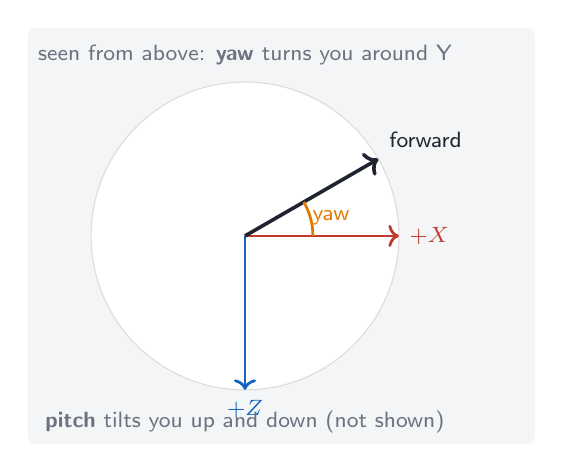
\begin{tikzpicture}[scale=1.15,every node/.style={font=\sffamily\footnotesize}]
  \fill[rlight,rounded corners=3pt] (-2.4,-2.3) rectangle (3.2,2.3);

  % ground circle (top view of yaw)
  \draw[codeframe,fill=white] (0,0) circle (1.7);
  \draw[->,rred,line width=1pt] (0,0) -- (1.7,0) node[right,text=rred] {$+X$};
  \draw[->,rblue,line width=1pt] (0,0) -- (0,-1.7) node[below,text=rblue] {$+Z$};

  \draw[->,rink,line width=1.3pt] (0,0) -- (30:1.7) node[above right,text=rink] {forward};
  \draw[rorange,line width=1pt] (0.75,0) arc (0:30:0.75);
  \node[text=rorange] at (0.95,0.2) {yaw};

  \node[align=left,text=rgrey] at (0,2.0) {seen from above: \textbf{yaw} turns you around Y};
  \node[align=left,text=rgrey] at (0,-2.05) {\textbf{pitch} tilts you up and down (not shown)};
\end{tikzpicture}
\end{center}

\begin{itemize}[leftmargin=*,itemsep=2pt]
  \item \textbf{yaw} --- the horizontal turn, spinning around the Y axis. Looking
        left and right.
  \item \textbf{pitch} --- the vertical tilt, around the X axis. Looking up and
        down.
\end{itemize}

There is a third, \emph{roll}, which tilts your head sideways. First person games
almost never use it, so we will not either.

Both are stored in \textbf{radians}, because that is what C's \lstinline|sinf|
and \lstinline|cosf| want. A full turn is $2\pi$. Convert for display with
raylib's \lstinline|RAD2DEG| and \lstinline|DEG2RAD| constants.

\section{From angles to a direction}

\begin{lstlisting}
Vector3 forward = {
    cosf(pitch)*cosf(yaw),
    sinf(pitch),
    cosf(pitch)*sinf(yaw)
};
\end{lstlisting}

If trigonometry is a distant memory, here is the intuition and you can leave it
at that. Ignore pitch for a second: on the flat ground, \lstinline|cos(yaw)| and
\lstinline|sin(yaw)| trace a circle of radius 1 as yaw goes round. That is the
direction you are facing, on the floor.

Now add pitch. \lstinline|sin(pitch)| is how much you are looking up, and it goes
straight into Y. \lstinline|cos(pitch)| shrinks the flat part: look straight up
and nothing is left of the horizontal direction, which is exactly right.

Starting value: \lstinline|yaw = -PI/2| points you along $-Z$, which is
conventionally ``into the screen''. \lstinline|pitch = 0| is the horizon.

\section{From a direction to sideways}

To strafe you need the direction to your right. That is the \textbf{cross
product} of where you are looking and where up is:

\begin{lstlisting}
Vector3 right = Vector3Normalize(
    Vector3CrossProduct(forward, (Vector3){ 0.0f, 1.0f, 0.0f }));
\end{lstlisting}

All you need to know about the cross product: give it two directions and it hands
back a third one perpendicular to both. Forward and up are perpendicular-ish, and
the thing perpendicular to both of them is sideways. That is the entire reason it
appears in every camera in existence.

\section{Moving}

\begin{lstlisting}
Vector3 flatForward = Vector3Normalize((Vector3){ forward.x, 0.0f, forward.z });

Vector3 move = { 0 };
if (IsKeyDown(KEY_W)) move = Vector3Add(move, flatForward);
if (IsKeyDown(KEY_S)) move = Vector3Subtract(move, flatForward);
if (IsKeyDown(KEY_D)) move = Vector3Add(move, right);
if (IsKeyDown(KEY_A)) move = Vector3Subtract(move, right);

if (Vector3Length(move) > 0.0f) move = Vector3Normalize(move);

camera.position = Vector3Add(camera.position, Vector3Scale(move, speed*dt));
camera.target   = Vector3Add(camera.position, forward);
\end{lstlisting}

That last line is the one that ties it all together: the camera looks at a point
one unit in front of the eye, in the direction we computed. Forget it and the
camera moves but never turns.

\section{The four details that make or break the feel}

\begin{enumerate}[leftmargin=*,itemsep=5pt]
  \item \textbf{Flatten the forward vector for walking.} Notice
        \lstinline|flatForward| above: the Y component is thrown away and the
        result renormalized. Without it, looking at the sky and pressing W makes
        you fly.

  \item \textbf{Clamp the pitch} to just under 90 degrees:
\begin{lstlisting}
if (pitch >  1.55f) pitch =  1.55f;     // about 89 degrees
if (pitch < -1.55f) pitch = -1.55f;
\end{lstlisting}
        At exactly 90, \lstinline|forward| is parallel to \lstinline|up|, the
        cross product collapses to zero, \lstinline|right| becomes undefined and
        the camera snaps violently. This is \emph{gimbal lock}, it is famous, and
        one \lstinline|if| avoids it.

  \item \textbf{Normalize the movement vector.} Hold W and D together without it
        and the two unit vectors add up to a length of $\sqrt{2}$: you move 41\%
        faster diagonally. Players find that exploit within a minute.

  \item \textbf{Multiply by \lstinline|dt|.} As always.
\end{enumerate}

\section{Reading the mouse}

\begin{lstlisting}
DisableCursor();                       // once, at startup

Vector2 mouse = GetMouseDelta();
yaw   += mouse.x*0.003f;
pitch -= mouse.y*0.003f;               // note the MINUS
\end{lstlisting}

Pitch subtracts because screen Y grows downwards while looking up is positive
pitch --- the 2D and 3D Y axes disagreeing one final time. Flip that sign and you
have inverted mouse look, which some people actually prefer, so make it an
option rather than a bug.

The \lstinline|0.003f| is mouse sensitivity, in radians per pixel. Expose it as a
setting; everybody wants a different one.

\section{The finishing touch: head bob}

Pure decoration, three lines, and it is most of what makes movement feel
physical:

\begin{lstlisting}
if (walking) bobTimer += dt*speed*1.6f;
float bob = walking ? sinf(bobTimer)*0.045f : 0.0f;
camera.position.y = EYE_HEIGHT + bob;
\end{lstlisting}

A sine wave on the eye height, running faster when you run. Keep the amplitude
tiny --- 4 centimetres is plenty. Anything bigger and players feel seasick.

\tryit{Lesson 4 of the 3D course is this chapter as a running program, printing
yaw, pitch and the forward vector live so you can watch the numbers as you turn.}{./course3d/build.sh 4}

\chapter{Collisions in 3D}

\section{The same idea, one more axis}

The 3D equivalent of a \lstinline|Rectangle| is an \textbf{AABB}: an
\emph{axis-aligned bounding box}. A box that never rotates, described by its two
opposite corners.

\begin{lstlisting}
typedef struct BoundingBox {
    Vector3 min;    // the corner with the smaller x, y and z
    Vector3 max;    // the corner with the larger  x, y and z
} BoundingBox;
\end{lstlisting}

And the rule is chapter 6's rule with a third line added: two boxes collide if
they overlap on \textbf{all three} axes at once.

\begin{lstlisting}
overlapX = (a.min.x <= b.max.x) && (a.max.x >= b.min.x);
overlapY = (a.min.y <= b.max.y) && (a.max.y >= b.min.y);
overlapZ = (a.min.z <= b.max.z) && (a.max.z >= b.min.z);
hit      = overlapX && overlapY && overlapZ;
\end{lstlisting}

raylib gives you it as \lstinline|CheckCollisionBoxes(a, b)|. Its relatives:

\begin{lstlisting}
CheckCollisionBoxes(boxA, boxB);
CheckCollisionSpheres(centreA, rA, centreB, rB);
CheckCollisionBoxSphere(box, centre, radius);
\end{lstlisting}

\section{Centre and size, not corners}

Nobody stores their objects as two corners. You store a position and a size, and
convert when you need to test:

\begin{lstlisting}
BoundingBox BoxFromCenter(Vector3 centre, Vector3 size)
{
    BoundingBox b;
    b.min = (Vector3){ centre.x - size.x/2, centre.y - size.y/2, centre.z - size.z/2 };
    b.max = (Vector3){ centre.x + size.x/2, centre.y + size.y/2, centre.z + size.z/2 };
    return b;
}
\end{lstlisting}

You will write this function in every 3D project you ever start. It is the same
``subtract half the size'' from chapter 3, with a z on the end.

\gotcha{The player's \lstinline|camera.position| is the height of their
\textbf{eyes}, not their middle. A 1.7 m person standing on the floor has eyes at
$Y = 1.7$ and a body centred at $Y = 0.85$. Build the collision box around the
body, not the eyes, or your player will collide with things at head height and
walk through everything below the knee.}

\begin{lstlisting}
Vector3 bodyCentre = { position.x, position.y - EYE_HEIGHT/2.0f, position.z };
Vector3 bodySize   = { RADIUS*2, EYE_HEIGHT, RADIUS*2 };
\end{lstlisting}

\section{Resolving, per axis, exactly as in 2D}

\begin{lstlisting}
Vector3 attempt = camera.position;
attempt.x += dx;
if (Collides(attempt)) { /* refused: keep the old x */ }
else camera.position.x = attempt.x;

attempt = camera.position;
attempt.z += dz;
if (Collides(attempt)) { /* refused: keep the old z */ }
else camera.position.z = attempt.z;
\end{lstlisting}

X then Z, because on foot those are the two ground axes. If you add jumping and
gravity, Y becomes a third pass with the same shape --- and the Y pass is where
you discover you have landed, because a refused downward move means there is
floor under you.

\keyidea{Detect with one call, resolve one axis at a time. It was true in 2D, it
is true in 3D, and it will still be true in whatever engine you use next.}

\section{Debugging: draw the boxes}

\begin{lstlisting}
DrawBoundingBox(playerBox, GREEN);
DrawBoundingBox(wallBox, hit ? RED : GREEN);
\end{lstlisting}

Nine times out of ten, a collision bug is not a logic bug --- the box is simply
not where you think it is. It is offset by half a height, or it is built from
last frame's position, or it is twice the size of the thing you drew. Draw it and
the bug is visible in a second instead of an hour.

\section{Grids: the other way, and the fast one}

Testing against a list of boxes is fine for a few dozen walls. For a whole level
there is a better approach, and it is what the original Doom did: store the level
as a \textbf{grid}, and convert a position straight into a cell index.

\begin{lstlisting}
static bool IsWall(float x, float z)
{
    int col = (int)floorf(x/CELL + 0.5f);
    int row = (int)floorf(z/CELL + 0.5f);

    if (col < 0 || col >= MAP_COLS || row < 0 || row >= MAP_ROWS) return true;

    return (MAP[row][col] == '#');
}
\end{lstlisting}

No loop. It costs the same whether the map has 10 walls or 10,000, and the
out-of-bounds check doubles as an invisible wall around the level.

To give the player some width, test the four corners of the square around them
instead of the single centre point:

\begin{lstlisting}
static bool CanStandAt(float x, float z)
{
    const float r = PLAYER_RADIUS;
    return !IsWall(x - r, z - r) && !IsWall(x + r, z - r)
        && !IsWall(x - r, z + r) && !IsWall(x + r, z + r);
}
\end{lstlisting}

\section{Shooting: rays}

A \lstinline|Ray| is a starting point and a direction:

\begin{lstlisting}
typedef struct Ray { Vector3 position; Vector3 direction; } Ray;
\end{lstlisting}

Fire one out of the camera and ask what it meets:

\begin{lstlisting}
Ray shot = { camera.position, forward };
RayCollision hit = GetRayCollisionBox(shot, EnemyBox(enemy.position));

if (hit.hit) { /* hit.distance, hit.point and hit.normal are filled in */ }
\end{lstlisting}

For a mouse click rather than a crosshair, build the ray from the cursor:

\begin{lstlisting}
Ray pick = GetScreenToWorldRay(GetMousePosition(), camera);
\end{lstlisting}

\gotcha{A ray goes on forever and hits everything in its path. To find what you
actually shot, loop over the candidates, keep the one with the smallest
\lstinline|hit.distance|, and compare it against the distance to the nearest
wall. Skip that last comparison and your players will happily shoot enemies
through solid walls.}

\tryit{Lesson 5 shows one box turning red on contact, with the three axis
overlaps printed separately; lesson 6 is a closed room where the walls actually
stop you.}{./course3d/build.sh 5 \quad and \quad ./course3d/build.sh 6}

\chapter{Building a silly little Doom}

Everything so far, assembled. The finished program is
\file{course3d/lesson07\_mini\_doom.c}: a corridor maze you walk through, enemies
that come after you, a gun that shoots them, and a HUD with a minimap. About 350
lines, and you have already met every idea in it.

\tryit{Run it first, then read this chapter with the source open next to
you.}{./course3d/build.sh 7}

\section{The level is a piece of text}

\begin{lstlisting}
static const char *MAP[MAP_ROWS] = {
    "###############",
    "#S....#.......#",
    "#.....#...E...#",
    "#.###.#.#####.#",
    ...
};
\end{lstlisting}

\lstinline|#| is a wall, \lstinline|.| is floor, \lstinline|S| is where the
player starts and \lstinline|E| is an enemy. Designing a level is now typing
characters into a text editor, and you can redesign the whole game in thirty
seconds. Plenty of shipped games stored their levels exactly like this.

\section{From map cell to world position}

The map is a grid of rows and columns. The world is metres along X, Y and Z. The
bridge between them is one function, and it is worth staring at until it is
obvious:

\begin{lstlisting}
static Vector3 CellToWorld(int col, int row, float y)
{
    return (Vector3){ col*CELL, y, row*CELL };
}
\end{lstlisting}

\begin{center}
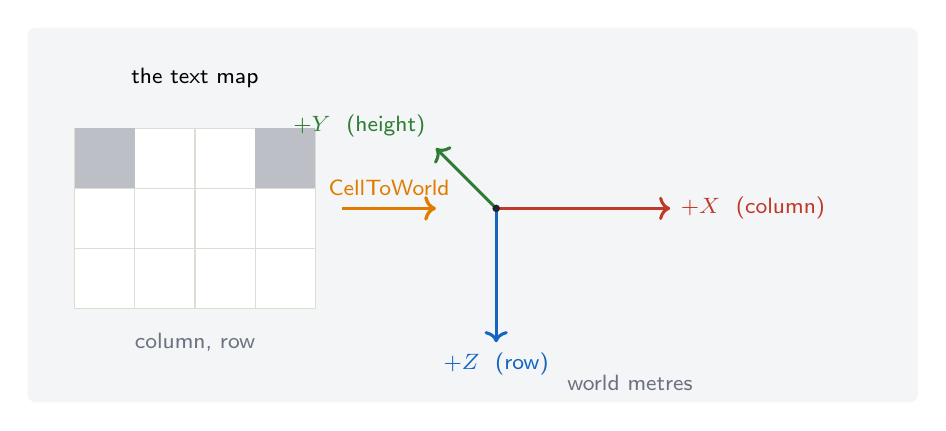
\begin{tikzpicture}[scale=0.85,every node/.style={font=\sffamily\footnotesize}]
  \fill[rlight,rounded corners=3pt] (-0.7,-4.1) rectangle (12.6,1.5);

  % grid
  \foreach \c in {0,1,2,3} \foreach \r in {0,1,2} {
    \draw[codeframe,fill=white] (\c*0.9,-\r*0.9) rectangle (\c*0.9+0.9,-\r*0.9-0.9);
  }
  \fill[rgrey!45] (0,0) rectangle (0.9,-0.9);
  \fill[rgrey!45] (0.9*3,0) rectangle (0.9*4,-0.9);
  \node at (1.8,0.75) {the text map};
  \node[text=rgrey] at (1.8,-3.2) {column, row};

  \draw[->,rorange,line width=1.2pt] (4.0,-1.2) -- (5.4,-1.2);
  \node[above,text=rorange] at (4.7,-1.15) {CellToWorld};

  % world
  \begin{scope}[xshift=6.3cm,yshift=-1.2cm]
    \draw[->,rred,line width=1.1pt] (0,0) -- (2.6,0) node[right,text=rred] {$+X$ \ (column)};
    \draw[->,rblue,line width=1.1pt] (0,0) -- (0,-2.0) node[below,text=rblue] {$+Z$ \ (row)};
    \draw[->,rgreen,line width=1.1pt] (0,0) -- (-0.9,0.9) node[above left,text=rgreen] {$+Y$ \ (height)};
    \fill[rink] (0,0) circle (1.6pt);
    \node[text=rgrey,align=left] at (2.0,-2.6) {world metres};
  \end{scope}
\end{tikzpicture}
\end{center}

\keyidea{Map \textbf{column} becomes world \textbf{X}. Map \textbf{row} becomes
world \textbf{Z}. Y is not in the map at all, because a top-down plan has no
height in it. This one mapping is the whole relationship between a 2D level
editor and a 3D world, and it runs backwards too --- that is how the minimap
turns a 3D position back into a dot.}

\section{Reading the map once, at startup}

\lstinline|ResetGame()| walks the text and turns markers into game state:

\begin{lstlisting}
for (int row = 0; row < MAP_ROWS; row++)
    for (int col = 0; col < MAP_COLS; col++)
    {
        if (MAP[row][col] == 'S')
            g->camera.position = CellToWorld(col, row, EYE_HEIGHT);
        else if (MAP[row][col] == 'E' && g->enemyCount < MAX_ENEMIES)
        {
            g->enemies[g->enemyCount].position = CellToWorld(col, row, 0.9f);
            g->enemies[g->enemyCount].alive = true;
            g->enemyCount++;
        }
    }
\end{lstlisting}

Because all the state lives in one \lstinline|Game| struct, restarting the level
is a single call to \lstinline|ResetGame(&game)| bound to the R key. Worth
copying as a habit: put the game state in a struct, write a reset function, and
you get restarts for free.

\section{The order of the frame}

The loop is one long sequence, and the order matters:

\begin{enumerate}[leftmargin=*,itemsep=2pt]
  \item \textbf{Look} --- mouse delta into yaw and pitch, pitch clamped, then
        build \lstinline|forward|, \lstinline|right| and
        \lstinline|flatForward| (chapter 12).
  \item \textbf{Move} --- keys into a direction, normalized, times speed times
        \lstinline|dt|, resolved one axis at a time against the grid
        (chapter 13).
  \item \textbf{Shoot} --- on click, fire a ray and see what it finds.
  \item \textbf{Enemies} --- walk towards the player, hurt them on contact.
  \item \textbf{Draw the world} --- inside \lstinline|BeginMode3D|.
  \item \textbf{Draw the HUD} --- after \lstinline|EndMode3D|, in screen pixels.
\end{enumerate}

Notice that all six steps read the same \lstinline|forward| vector that step 1
computed. Compute it once per frame, near the top, and pass it around. Computing
it twice with different values is how you get a gun that shoots slightly to the
left of the crosshair.

\section{Walls}

One cube per \lstinline|#| cell, with a shade that varies by position so the
corridors do not look like a single flat mass:

\begin{lstlisting}
Vector3 centre = CellToWorld(col, row, WALL_HEIGHT/2);
int shade = 88 + ((col*7 + row*13) % 26);
DrawCube(centre, CELL, WALL_HEIGHT, CELL, wall);
DrawCubeWires(centre, CELL, WALL_HEIGHT, CELL, (Color){ 30, 26, 24, 255 });
\end{lstlisting}

Note \lstinline|WALL_HEIGHT/2| for the Y: the cube's centre is at half its
height, so it sits on the floor instead of sinking into it (chapter 9).

Floor and ceiling are two \lstinline|DrawPlane| calls in different colours. Two
lines, and suddenly you are indoors.

\section{Shooting}

\begin{lstlisting}
Ray shot = { game.camera.position, forward };

// how far is the wall in front of us?
float wallDistance = 100.0f;
for (float t = 0.1f; t < 60.0f; t += 0.1f)
{
    Vector3 p = Vector3Add(shot.position, Vector3Scale(shot.direction, t));
    if (IsWall(p.x, p.z)) { wallDistance = t; break; }
}

// the nearest enemy closer than that wall
int target = -1;
float best = wallDistance;

for (int i = 0; i < game.enemyCount; i++)
{
    if (!game.enemies[i].alive) continue;
    RayCollision hit = GetRayCollisionBox(shot, EnemyBox(game.enemies[i].position));
    if (hit.hit && hit.distance < best) { best = hit.distance; target = i; }
}
\end{lstlisting}

Two things are happening. The loop marching along the ray in 10 cm steps is a
crude \emph{raycast} against the grid --- it walks forward until it is inside a
wall cell, and that is your line of sight. Seeding \lstinline|best| with that
distance is what stops you shooting through walls: an enemy only counts if it is
nearer than the wall.

\gotcha{Stepping along a ray in fixed increments can step straight over a thin
wall if the step is bigger than the wall. Ours is 10 cm against 2 m walls, so it
is safe. Proper raycasters use a grid traversal algorithm (look up ``DDA'') that
cannot miss, and that is the next thing to learn if you want to go further down
this road.}

\section{Enemies}

The simplest AI that still feels like a game: if you can see me and I am not
touching you, walk at you.

\begin{lstlisting}
Vector3 toPlayer = Vector3Subtract(game.camera.position, e->position);
toPlayer.y = 0.0f;                       // ignore height: they walk, not fly
float distance = Vector3Length(toPlayer);

if (distance < 12.0f && distance > 0.9f)
{
    Vector3 step = Vector3Scale(Vector3Normalize(toPlayer), 1.6f*dt);
    if (CanStandAt(e->position.x + step.x, e->position.z)) e->position.x += step.x;
    if (CanStandAt(e->position.x, e->position.z + step.z)) e->position.z += step.z;
}
else if (distance <= 0.9f)
{
    game.health -= 25.0f*dt;             // four seconds of contact kills you
}
\end{lstlisting}

The pattern \lstinline|normalize(target - me) * speed * dt| is how absolutely
everything chases everything else: enemies, homing missiles, a pet following you.
Learn it once, use it forever.

Their movement is resolved per axis too --- same two lines as the player --- so
they slide along walls instead of getting stuck in corners.

\section{The HUD, or where the 2D course pays off}

Everything after \lstinline|EndMode3D()| is plain screen pixels:

\begin{itemize}[leftmargin=*,itemsep=3pt]
  \item \textbf{Crosshair} --- four short \lstinline|DrawLine| calls with a gap
        in the middle, centred on \lstinline|GetScreenWidth()/2|.
  \item \textbf{The gun} --- three rectangles at the bottom of the screen, offset
        by the same \lstinline|sinf(bobTimer)| that bobs the camera, so the
        weapon sways with your steps. A muzzle flash is two circles drawn for
        0.06 seconds after a shot.
  \item \textbf{Health bar} --- a background rectangle and a second one whose
        width is \lstinline|224.0f*health/100.0f|, turning red below 30.
  \item \textbf{Minimap} --- the text map drawn as little squares, with the
        player and enemies as dots. World X divided by the cell size gives the
        map column, which gives the screen X. Chapter 9's ``the floor is XZ''
        used in reverse.
\end{itemize}

\begin{lstlisting}
int px = ox + (int)(game.camera.position.x/CELL*tile);
int py = oy + (int)(game.camera.position.z/CELL*tile);
DrawCircle(px, py, 3, SKYBLUE);
DrawLine(px, py, px + (int)(forward.x*14), py + (int)(forward.z*14), SKYBLUE);
\end{lstlisting}

That last line is the little arrow showing which way you face: the 3D forward
vector, with its Y thrown away, drawn as a 2D line. Three dimensions and two
dimensions, in the same frame, sharing one number.

\section{Things to change first}

The point of having the source is breaking it. In rough order of fun per minute:

\begin{enumerate}[leftmargin=*,itemsep=2pt]
  \item Redraw the map. Add a room, a dead end, a long corridor.
  \item Change \lstinline|WALL_HEIGHT| to 8 and walk around. Then try 1.5.
  \item Set \lstinline|fovy| to 110 and then to 40. Feel how much the lens
        changes the game.
  \item Give the enemies different speeds, or make them stop when they are far
        away and only wake when they see you.
  \item Add a pickup: a \lstinline|P| in the map, drawn as a spinning cube
        (rotate it with \lstinline|GetTime()|), that refills ammo when you touch
        it. Everything you need is in chapters 9 and 13.
  \item Add jumping: a \lstinline|velocityY|, gravity subtracted every frame, and
        the Y axis resolved like X and Z.
\end{enumerate}

\part{The rest of the library}

\chapter{Sound and music}

Of everything left in the library, this is the one that changes how finished your
game feels for the least work. Three function calls and the mini Doom stops being
a tech demo.

\section{One line before anything}

\begin{lstlisting}
InitAudioDevice();      // right after InitWindow
...
CloseAudioDevice();     // right before CloseWindow
\end{lstlisting}

Nothing in raudio works before that call, exactly like \lstinline|InitWindow| for
graphics. If sounds silently do nothing, check this first.

\section{The four things raudio gives you}

\begin{center}
\begin{tabular}{@{}llp{6.4cm}@{}}
\toprule
\textbf{Type} & \textbf{Lives} & \textbf{Use it for} \\
\midrule
\lstinline|Wave| & in RAM, raw samples & building or editing audio yourself \\
\lstinline|Sound| & in RAM, decoded & short clips: gunshots, steps, clicks \\
\lstinline|Music| & streamed from disk & long tracks: the soundtrack \\
\lstinline|AudioStream| & you push samples & synthesisers, anything procedural \\
\bottomrule
\end{tabular}
\end{center}

The split between \lstinline|Sound| and \lstinline|Music| is about memory. A
three minute track decoded into RAM is around 30 MB; streamed, it costs a few
kilobytes of buffer. A footstep is 4 KB either way, so it may as well be resident
and instant.

\section{Sounds}

\begin{lstlisting}
Sound shot = LoadSound("shot.wav");      // once, outside the loop

if (IsMouseButtonPressed(MOUSE_BUTTON_LEFT)) PlaySound(shot);

UnloadSound(shot);                       // once, after the loop
\end{lstlisting}

Same load-outside, unload-after rule as textures. raylib reads \file{.wav},
\file{.ogg}, \file{.mp3}, \file{.flac}, \file{.qoa} and a few more.

\lstinline|PlaySound| does not wait and does not queue --- it fires and returns
immediately. Call it twice in one frame and you get two overlapping copies, which
is exactly what you want for gunfire.

\subsection{The trick that makes repeated sounds bearable}

A sound effect played identically fifty times in ten seconds becomes torture.
Real games vary it slightly on every shot:

\begin{lstlisting}
SetSoundPitch(shot, 0.85f + GetRandomValue(0, 30)/100.0f);
SetSoundPan(shot, GetRandomValue(20, 80)/100.0f);
PlaySound(shot);
\end{lstlisting}

Pitch is a multiplier, so 1.0 is unchanged and 0.5 is an octave down. Pan runs
0.0 (left) to 1.0 (right), with 0.5 centred.

\gotcha{\lstinline|SetSoundPitch| changes that \lstinline|Sound| object for
every future play, not just the next one. If you want two enemies to sound
different at the same time you need \lstinline|LoadSoundAlias()|, which shares
the samples but gives you a second set of playback settings, and costs almost
nothing.}

\section{Music}

\begin{lstlisting}
Music track = LoadMusicStream("theme.ogg");
track.looping = true;
PlayMusicStream(track);

while (!WindowShouldClose())
{
    UpdateMusicStream(track);     // <-- EVERY FRAME. Not optional.
    ...
}

UnloadMusicStream(track);
\end{lstlisting}

\gotcha{\lstinline|UpdateMusicStream()| is the single most forgotten call in
raylib. It refills the streaming buffer from disk. Miss it and your music plays
for a fraction of a second and stops --- no error, no warning, just silence. If
music ``does not work'', this is the reason nine times out of ten.}

Pause, resume and seek behave as you would expect, and two getters let you draw a
progress bar:

\begin{lstlisting}
PauseMusicStream(track);  ResumeMusicStream(track);  StopMusicStream(track);
SeekMusicStream(track, 30.0f);                        // jump to 30 seconds

float played = GetMusicTimePlayed(track);
float length = GetMusicTimeLength(track);
\end{lstlisting}

\section{Making sounds with no sound files}

You do not need an artist to get started. A \lstinline|Wave| is just numbers, and
a 16-bit mono wave is one \lstinline|short| per sample, from $-32768$ to $32767$:

\begin{lstlisting}
Wave wave = { 0 };
wave.sampleRate = 44100;      // samples per second
wave.sampleSize = 16;         // bits per sample
wave.channels   = 1;          // mono
wave.frameCount = 44100/5;    // a fifth of a second

short *samples = (short *)MemAlloc(wave.frameCount*sizeof(short));

float phase = 0.0f;
for (unsigned int i = 0; i < wave.frameCount; i++)
{
    float t = (float)i/wave.frameCount;        // 0..1 through the sound
    float hz = 1400.0f + (200.0f - 1400.0f)*t; // pitch slides DOWN
    phase += 2.0f*PI*hz/44100.0f;

    float envelope = (1.0f - t)*(1.0f - t);    // fade out, or it clicks
    samples[i] = (short)(sinf(phase)*envelope*22000.0f);
}

wave.data = samples;
Sound laser = LoadSoundFromWave(wave);
\end{lstlisting}

Three ideas are doing all the work there, and they are the whole of retro sound
design:

\begin{itemize}[leftmargin=*,itemsep=3pt]
  \item \textbf{A sine wave} gives you a pure tone. \lstinline|phase| accumulates
        and \lstinline|sinf(phase)| oscillates.
  \item \textbf{Sliding the pitch} turns a beep into a laser (down) or a power-up
        (up).
  \item \textbf{An envelope} --- multiplying by a value that falls to zero ---
        makes it a sound instead of a rude noise. Without a fade-out, the sound
        stops mid-oscillation and the speaker cone jumps, which you hear as a
        click.
\end{itemize}

Mix in random noise instead of a sine and you have an explosion. That is
literally what the \textbf{rFXGen} tool on raylib.com does, with sliders.

\gotcha{Use \lstinline|MemAlloc()| rather than \lstinline|malloc()| for wave
data. \lstinline|UnloadWave()| frees it with raylib's allocator, and mixing
allocators is the kind of bug that crashes only on some machines.}

\subsection{Wave and Sound are two separate allocations}

\lstinline|LoadSoundFromWave| copies the samples to the audio device. The
original \lstinline|Wave| is still yours, and still needs freeing:

\begin{lstlisting}
UnloadSound(laser);
UnloadWave(wave);      // both, not one
\end{lstlisting}

You can also write it out --- \lstinline|ExportWave(wave, "laser.wav")| --- which
is a genuinely useful way to build a sound in code, listen to it, and then ship
the file.

\section{Audio streams, for sound you generate live}

When the samples cannot exist ahead of time --- a synthesiser, an engine note
that follows the revs, voice chat --- you push them yourself:

\begin{lstlisting}
AudioStream stream = LoadAudioStream(44100, 16, 1);
PlayAudioStream(stream);

// in the loop:
if (IsAudioStreamProcessed(stream))     // the device wants more
{
    static short chunk[4096];
    for (int i = 0; i < 4096; i++) { phase += step; chunk[i] = ...; }
    UpdateAudioStream(stream, chunk, 4096);
}
\end{lstlisting}

The contract is: ask whether a buffer has been consumed, and if so, hand over the
next one. Miss the window and you hear a gap.

\section{Volume, and being polite}

\begin{lstlisting}
SetMasterVolume(0.6f);            // everything
SetSoundVolume(shot, 0.4f);       // one sound
SetMusicVolume(track, 0.5f);      // one track
\end{lstlisting}

Ship with the master volume somewhere around 0.5 and put it in an options menu.
Players will forgive almost anything except a game that is deafening on the first
launch.

\tryit{Module 9 synthesises a beep, a laser and an explosion in C, writes a
four second tune to a real \file{.wav} and streams it back, and lets you play a
live tone with the mouse controlling the pitch. No audio files
involved.}{./cheatsheet/build.sh 9}

\chapter{Shaders, and why your cubes look flat}

Chapter 11 told you that plain \lstinline|DrawCube| does no lighting, and left it
there. This is the chapter that explains what to do about it.

\section{What a shader actually is}

A shader is a small program that runs \textbf{on the GPU}, in parallel, an
absurd number of times per frame. You write it in GLSL, a C-like language, and
you get two of them:

\begin{center}
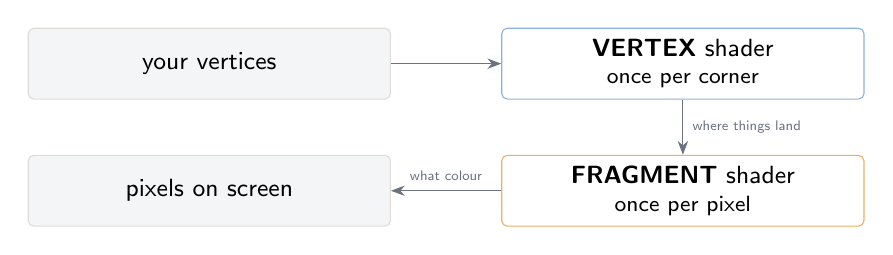
\begin{tikzpicture}[
  node distance=7mm,
  every node/.style={font=\sffamily\small},
  bx/.style={draw=codeframe,fill=rlight,rounded corners=2pt,minimum width=4.6cm,minimum height=9mm,align=center},
  arrow/.style={-{Stealth[length=5pt]},rgrey}
]
\node[bx] (verts) {your vertices};
\node[bx,right=14mm of verts,fill=white,draw=rblue!50] (vs) {\textbf{VERTEX} shader\\[-1pt]{\footnotesize once per corner}};
\node[bx,below=of vs,fill=white,draw=rorange!60] (fs) {\textbf{FRAGMENT} shader\\[-1pt]{\footnotesize once per pixel}};
\node[bx,left=14mm of fs] (screen) {pixels on screen};
\draw[arrow] (verts) -- (vs);
\draw[arrow] (vs) -- node[right,font=\sffamily\tiny,text=rgrey] {where things land} (fs);
\draw[arrow] (fs) -- node[above,font=\sffamily\tiny,text=rgrey] {what colour} (screen);
\end{tikzpicture}
\end{center}

\begin{itemize}[leftmargin=*,itemsep=3pt]
  \item The \textbf{vertex} shader runs once per corner of your geometry and
        decides \emph{where} it lands on screen.
  \item The \textbf{fragment} shader runs once per pixel and decides \emph{what
        colour} that pixel is.
\end{itemize}

At 1080p a fullscreen effect runs your fragment shader two million times, sixty
times a second. That is why it must be tiny and why it cannot talk back to your
C code.

\keyidea{raylib ships a default pair that just draws things normally. You almost
always write only the fragment shader and pass \lstinline|NULL| for the vertex
one. Lighting, colour grading, outlines, water, fog --- all fragment shaders.}

\section{The three steps, which never change}

\begin{lstlisting}
// 1. LOAD, once, outside the loop
Shader shader = LoadShader(NULL, "glow.fs");          // from files
Shader shader = LoadShaderFromMemory(NULL, fsCode);   // from a string

// 2. FIND THE SLOTS, once: a lookup by name into the compiled program
int locTime = GetShaderLocation(shader, "uTime");

// 3. FEED AND USE, every frame
SetShaderValue(shader, locTime, &time, SHADER_UNIFORM_FLOAT);

BeginShaderMode(shader);
    DrawTexture(tex, 0, 0, WHITE);     // drawn THROUGH the shader
EndShaderMode();
\end{lstlisting}

That \lstinline|Begin|/\lstinline|End| pair is the same contract as the cameras:
inside it, the shader applies; outside, normal drawing. Your HUD goes outside,
for the same reason as always.

\section{Uniforms: the only way to talk to the GPU}

A \emph{uniform} is a variable you send from C into the shader. It is called
uniform because it has the same value for every pixel in that draw call.

\begin{center}
\begin{tabular}{@{}ll@{}}
\toprule
\textbf{C side} & \textbf{GLSL side} \\
\midrule
\lstinline|SHADER_UNIFORM_FLOAT| & \lstinline|uniform float uTime;| \\
\lstinline|SHADER_UNIFORM_VEC2| & \lstinline|uniform vec2 uLight;| \\
\lstinline|SHADER_UNIFORM_VEC3| & \lstinline|uniform vec3 uColour;| \\
\lstinline|SHADER_UNIFORM_INT| & \lstinline|uniform int uMode;| \\
\lstinline|SetShaderValueTexture| & \lstinline|uniform sampler2D uSecond;| \\
\bottomrule
\end{tabular}
\end{center}

\gotcha{\lstinline|GetShaderLocation| returns $-1$ if the name is not found ---
and GLSL compilers \emph{delete unused uniforms}, so a uniform you declared but
never read in the shader body will not be there. A silent $-1$ that makes
\lstinline|SetShaderValue| do nothing is the classic first shader bug.}

\section{A fragment shader, line by line}

\begin{lstlisting}[style=plain]
#version 330

in vec2 fragTexCoord;             // from the vertex shader: where we are, 0..1
in vec4 fragColor;                // the tint passed to DrawTexture

uniform sampler2D texture0;       // the texture raylib binds automatically
uniform vec4 colDiffuse;          // raylib's diffuse colour

out vec4 finalColor;              // what we must write

void main()
{
    vec4 texel = texture(texture0, fragTexCoord)*colDiffuse*fragColor;
    float grey = dot(texel.rgb, vec3(0.299, 0.587, 0.114));
    finalColor = vec4(grey, grey, grey, texel.a);
}
\end{lstlisting}

Four things to notice:

\begin{enumerate}[leftmargin=*,itemsep=3pt]
  \item \lstinline|#version 330| must be the very first thing in the file or
        string. Not a comment, not a blank line. On desktop raylib uses GLSL 330.
  \item \lstinline|texture0|, \lstinline|colDiffuse|, \lstinline|fragTexCoord|
        and \lstinline|fragColor| are names raylib fills in for you. Spell them
        exactly or you get nothing.
  \item \lstinline|vec4| is four floats, and colours here run \textbf{0.0 to
        1.0}, not 0 to 255.
  \item The last line of the function must write \lstinline|finalColor|. That is
        the shader's entire output.
\end{enumerate}

Those weights \lstinline|(0.299, 0.587, 0.114)| are how bright each channel looks
to a human eye --- green far more than blue. Averaging the three instead gives a
muddy grey, which is why this particular triple turns up everywhere.

\section{Errors show up at run time, not compile time}

Your C compiles fine whatever nonsense is in the shader string: the GPU compiler
only runs when \lstinline|LoadShader| executes. Watch the terminal:

\begin{lstlisting}[style=plain]
INFO: SHADER: [ID 5] Fragment shader compiled successfully
INFO: SHADER: [ID 6] Program shader loaded successfully
\end{lstlisting}

If instead you see \lstinline|SHADER: [ID 5] Failed to compile fragment shader|,
the line number in the message refers to the \emph{shader} source. A failed
shader falls back to the default one, so your scene keeps rendering normally and
the only sign of trouble is that your effect does nothing.

\section{Lighting, honestly}

Real lighting is a fragment shader that receives the surface normal and the light
positions, and computes how much each light hits each pixel. raylib does not
build that in --- the \file{examples/shaders/} folder has it, in
\file{shaders\_basic\_lighting.c}, as about 80 lines of GLSL.

Before you go there, be aware of the cheaper options from chapter 11: wireframes
over solid shapes, colour variation per object, and a distinct floor and ceiling.
They cost nothing, they work everywhere, and plenty of good-looking games never
do anything more.

\keyidea{Learn shaders when flat colour is actually holding your game back, not
before. It is the deepest rabbit hole in graphics and the easiest place to spend
three weeks and ship nothing.}

\tryit{Module 3 has three fragment shaders written as C strings --- greyscale, a
wave distortion driven by a \lstinline|uTime| uniform, and a spotlight that
follows your mouse. The HUD is drawn outside the pair so you can see what the
shader does and does not touch.}{./cheatsheet/build.sh 3}

\chapter{Meshes, models and materials}

Chapter 11 drew everything with \lstinline|DrawCube| and friends. Those are
throwaways: they build geometry from scratch every frame and cannot carry a
texture. This chapter is the step up.

\section{The three layers}

\begin{center}
\begin{tabular}{@{}lp{9.2cm}@{}}
\toprule
\textbf{\lstinline|Mesh|} & raw geometry: vertex positions, normals, texture
coordinates. Lives on the GPU. No colour, no texture. \\[3pt]
\textbf{\lstinline|Material|} & how a surface looks: a shader plus a set of
texture maps (diffuse, normal, roughness\ldots) and a tint. \\[3pt]
\textbf{\lstinline|Model|} & one or more meshes, one or more materials, and a
transform matrix tying them together. \\
\bottomrule
\end{tabular}
\end{center}

A model loaded from a \file{.glb} file arrives with all three filled in. When you
build one yourself, you assemble them:

\begin{lstlisting}
Mesh mesh   = GenMeshCube(2.0f, 2.0f, 2.0f);
Model model = LoadModelFromMesh(mesh);          // wraps it, default white material
\end{lstlisting}

\section{Generating geometry}

You do not need a modelling program to get real meshes:

\begin{center}
\begin{tabular}{@{}ll@{}}
\toprule
\lstinline|GenMeshCube(w, h, l)| & a box \\
\lstinline|GenMeshSphere(radius, rings, slices)| & more rings = smoother, slower \\
\lstinline|GenMeshPlane(w, l, resX, resZ)| & a floor; resolution matters if you deform it \\
\lstinline|GenMeshCylinder(radius, height, slices)| & pillars, trees, barrels \\
\lstinline|GenMeshTorus(radius, size, rad, sides)| & a doughnut \\
\lstinline|GenMeshKnot(...)| & a torus knot, for showing off \\
\lstinline|GenMeshHeightmap(image, size)| & \textbf{terrain from a greyscale image} \\
\lstinline|GenMeshCubicmap(image, size)| & \textbf{a 3D maze from a pixel map} \\
\bottomrule
\end{tabular}
\end{center}

Those last two deserve attention. \lstinline|GenMeshHeightmap| turns a greyscale
picture into hills, where brightness is altitude. \lstinline|GenMeshCubicmap|
turns a black-and-white pixel map into walls --- it is the mini Doom's text map,
except it produces a single mesh instead of hundreds of separate cubes, so it
draws in one call instead of two hundred.

\section{Putting a texture on something}

This is the thing \lstinline|DrawCube| cannot do:

\begin{lstlisting}
Texture2D tex = LoadTexture("wall.png");
model.materials[0].maps[MATERIAL_MAP_DIFFUSE].texture = tex;
\end{lstlisting}

Read it inside out: the model's first material, its diffuse map, its texture.
\lstinline|MATERIAL_MAP_DIFFUSE| is the plain colour map; there are slots for
normal maps, roughness, occlusion and the rest, which only matter once you have a
shader that reads them.

You can tint per draw as well, and the two multiply:

\begin{lstlisting}
DrawModel(model, position, 1.0f, WHITE);    // texture as-is
DrawModel(model, position, 1.0f, RED);      // texture tinted red
\end{lstlisting}

\section{Drawing}

\begin{lstlisting}
DrawModel(model, position, scale, tint);
DrawModelEx(model, position, rotationAxis, rotationAngle, scaleVec3, tint);
DrawModelWires(model, position, scale, tint);
DrawBoundingBox(GetMeshBoundingBox(mesh), GREEN);
\end{lstlisting}

\lstinline|DrawModelEx| is the one you want for anything that turns: an axis, an
angle in degrees, and a per-axis scale.

\begin{lstlisting}
DrawModelEx(model, pos, (Vector3){ 0, 1, 0 }, angle, (Vector3){ 1, 1, 1 }, WHITE);
\end{lstlisting}

Rotating around \lstinline|(0,1,0)| means spinning about the vertical axis, which
is what you want for a character turning or a pickup idling.

\section{Loading real models}

\begin{lstlisting}
Model robot = LoadModel("robot.glb");       // once
DrawModel(robot, position, 1.0f, WHITE);    // every frame
UnloadModel(robot);                         // once
\end{lstlisting}

raylib reads \file{.obj}, \file{.gltf}, \file{.glb}, \file{.iqm}, \file{.m3d} and
\file{.vox}. Prefer \textbf{\file{.glb}}: it packs the mesh, the materials and the
textures into one file, so there is nothing to go missing and no paths to fix.

\gotcha{\lstinline|UnloadModel| frees the meshes it owns but deliberately does
\emph{not} free textures or shaders --- you might be sharing them between models,
so raylib leaves them to you. Unload your textures yourself, exactly once.}

\section{Animation}

\begin{lstlisting}
int animCount = 0;
ModelAnimation *anims = LoadModelAnimations("robot.glb", &animCount);
int frame = 0;

// in the loop:
frame = (frame + 1) % anims[0].frameCount;
UpdateModelAnimation(robot, anims[0], frame);
DrawModel(robot, position, 1.0f, WHITE);

UnloadModelAnimations(anims, animCount);
\end{lstlisting}

The model must have been exported with a skeleton, \file{.glb} and \file{.iqm}
being the usual choices. Note that stepping \lstinline|frame| once per frame ties
the animation to your frame rate --- use a timer, as in chapter 5, if you care.

\section{Billboards: the old trick, still useful}

A billboard is a flat image that always turns to face the camera. Every enemy in
Doom was one.

\begin{lstlisting}
DrawBillboard(camera, texture, position, size, WHITE);
DrawBillboardRec(camera, texture, sourceRec, position, size, WHITE);  // one sprite of a sheet
\end{lstlisting}

They are cheap, they look deliberately retro, and \lstinline|DrawBillboardRec|
lets you animate them from a sprite sheet exactly as in chapter 7. For particles,
smoke, flames and pickups they are still the right answer today.

\section{When to stop using DrawCube}

\begin{center}
\begin{tabular}{@{}ll@{}}
\toprule
\textbf{Stay with immediate shapes if} & \textbf{Move to models when} \\
\midrule
prototyping & you want textures \\
a handful of objects & you want lighting via a shader \\
debug visualisation & you draw hundreds of the same thing \\
flat colour is fine & you need animation \\
\bottomrule
\end{tabular}
\end{center}

And when you are drawing the same mesh thousands of times --- grass, crowds,
asteroids --- there is \lstinline|DrawMeshInstanced|, which sends one mesh and an
array of transforms in a single call. It is the difference between 50 FPS and
2000.

\tryit{Module 8 generates a cube, a sphere and a torus, puts a generated
checkerboard on the cube's material, draws a billboard, and lets you click any
object to pick it with a ray. TAB switches between models, immediate shapes and
wireframe so you can compare them.}{./cheatsheet/build.sh 8}

\chapter{Images, render textures and colour}

Chapter 7 covered enough of rtextures to draw a sprite. This is the rest of the
module: editing pixels, drawing into textures, and the colour helpers.

\section{Image work happens on the CPU}

An \lstinline|Image| is pixels in ordinary RAM, and raylib gives you a small
image editor's worth of functions to work on them:

\begin{center}
\begin{tabular}{@{}ll@{}}
\toprule
\lstinline|ImageResize / ImageResizeNN| & smooth, or nearest-neighbour for pixel art \\
\lstinline|ImageCrop / ImageAlphaCrop| & cut a region, or trim transparent edges \\
\lstinline|ImageFlipHorizontal / Vertical| & mirror \\
\lstinline|ImageRotate / ImageRotateCW| & turn \\
\lstinline|ImageColorTint / Invert / Grayscale| & recolour every pixel \\
\lstinline|ImageColorBrightness / Contrast| & adjust \\
\lstinline|ImageColorReplace| & swap one exact colour for another \\
\lstinline|ImageDrawRectangle / Circle / Text| & \textbf{draw into the image} \\
\lstinline|ImageDraw| & paste one image into another \\
\lstinline|ImageFormat| & convert the pixel layout \\
\bottomrule
\end{tabular}
\end{center}

\gotcha{Almost all of these take a \lstinline|Image *| and modify it in place ---
\lstinline|ImageResize(&img, 128, 128)|, not \lstinline|img = ImageResize(...)|.
And they all work on the CPU, so they are far too slow to run every frame. Do
them once at load time, then upload.}

Use \lstinline|ImageCopy| before editing if you want to keep the original.

\section{Generating images from nothing}

\begin{lstlisting}
GenImageColor(w, h, colour);                      // a flat fill
GenImageGradientLinear(w, h, angle, a, b);        // a linear gradient
GenImageGradientRadial(w, h, density, a, b);      // a radial one: glows, vignettes
GenImageChecked(w, h, cw, ch, a, b);              // a checkerboard
GenImageWhiteNoise(w, h, factor);                 // static
GenImagePerlinNoise(w, h, offX, offY, scale);     // smooth noise: terrain, clouds
GenImageCellular(w, h, tileSize);                 // organic cell patterns
\end{lstlisting}

This is how you get a game looking like something before an artist exists.
\lstinline|GenImagePerlinNoise| feeding \lstinline|GenMeshHeightmap| from the
last chapter gives you an entire landscape in four lines.

\section{Render textures: drawing into a texture}

A \lstinline|RenderTexture2D| is a texture you can draw into, with its own
Begin/End pair:

\begin{lstlisting}
RenderTexture2D canvas = LoadRenderTexture(320, 240);     // once

// in the loop, BEFORE BeginDrawing:
BeginTextureMode(canvas);
    ClearBackground(BLACK);
    DrawCircle(160, 120, 40, ORANGE);
EndTextureMode();

BeginDrawing();
    DrawTexture(canvas.texture, 0, 0, WHITE);
EndDrawing();

UnloadRenderTexture(canvas);                              // once
\end{lstlisting}

This unlocks four things you cannot do otherwise:

\begin{enumerate}[leftmargin=*,itemsep=3pt]
  \item \textbf{Pixel-art at a fixed resolution.} Render your game at 320$\times$180
        and scale it up to the window. Every pixel stays square and crisp, at any
        window size.
  \item \textbf{A real minimap.} Draw the world from a top-down camera into a
        texture, then draw that texture in the corner.
  \item \textbf{Fullscreen shader effects.} Render the scene into a texture, then
        draw that texture through a shader. Bloom, colour grading, blur --- all
        of it works this way.
  \item \textbf{In-world screens.} Security monitors, mirrors, portals.
\end{enumerate}

\gotcha{A render texture comes out \textbf{upside down}, because OpenGL's Y axis
points the other way. The fix is a negative height in the source rectangle:

\lstinline|(Rectangle){ 0, 0, (float)rt.texture.width, -(float)rt.texture.height }|

Use \lstinline|DrawTexturePro| or \lstinline|DrawTextureRec| with that, and never
plain \lstinline|DrawTexture|, or your scene is mirrored vertically.}

\section{Texture filters and mipmaps}

\begin{lstlisting}
SetTextureFilter(tex, TEXTURE_FILTER_POINT);        // crisp: pixel art
SetTextureFilter(tex, TEXTURE_FILTER_BILINEAR);     // smooth: photos, 3D
GenTextureMipmaps(&tex);
SetTextureFilter(tex, TEXTURE_FILTER_TRILINEAR);    // smooth + mipmaps
\end{lstlisting}

\lstinline|POINT| is what makes pixel art look like pixel art; the default
bilinear filter will blur your beautiful 16$\times$16 sprite into mush the moment
you scale it.

Mipmaps are pre-shrunk copies of a texture. Without them, a wall texture seen
from far away shimmers as you walk, because each pixel is sampling a random spot
in the full-size image. Generate them for anything in a 3D world; skip them for
2D sprites drawn at their real size.

\section{Colour helpers}

\begin{center}
\begin{tabular}{@{}ll@{}}
\toprule
\lstinline|Fade(colour, 0.5f)| & same colour, half alpha \\
\lstinline|ColorTint(colour, tint)| & multiply two colours \\
\lstinline|ColorBrightness(colour, -0.4f)| & $-1$ black, $+1$ white \\
\lstinline|ColorContrast(colour, 0.5f)| & \\
\lstinline|ColorAlphaBlend(dst, src, tint)| & blend as if drawn on top \\
\lstinline|ColorLerp(a, b, t)| & blend two colours \\
\lstinline|ColorToHSV / ColorFromHSV| & hue, saturation, value \\
\lstinline|ColorToInt / GetColor| & to and from \lstinline|0xRRGGBBAA| \\
\bottomrule
\end{tabular}
\end{center}

HSV is the one worth knowing about. Shifting only the hue gives you a whole
palette of related colours --- team colours, damage states, day and night --- from
a single base:

\begin{lstlisting}
Vector3 hsv = ColorToHSV(base);
Color enemyTeam = ColorFromHSV(hsv.x + 180, hsv.y, hsv.z);   // opposite hue
\end{lstlisting}

And \lstinline|GetColor(0x1F2430FF)| lets you paste hex values straight from a
design tool, which is more pleasant than counting bytes.

\tryit{Module 6 shows all six image generators, a chain of CPU edits, the four
ways to draw a texture, a live render texture with its flipped source rectangle,
and the colour helpers side by side.}{./cheatsheet/build.sh 6}

\chapter{Fonts and text}

\lstinline|DrawText| with the built-in font gets you through a prototype. The
moment you want a game that looks designed, you need the rest of rtext.

\section{Loading a font properly}

\begin{lstlisting}
Font font = LoadFont("kenney.ttf");                     // default size 32
Font font = LoadFontEx("kenney.ttf", 48, NULL, 0);      // the one you want
\end{lstlisting}

\lstinline|LoadFontEx| takes the size to rasterise at, and optionally a list of
codepoints to include. Passing \lstinline|NULL, 0| gives you the default set of
95 ASCII characters.

\gotcha{A font is baked into a bitmap at \textbf{one fixed size}. Load it at 16
and draw it at 64 and it will be blurry --- that is not a bug, it is a small
image being stretched. Load it at, or slightly above, the largest size you will
actually draw.}

For accented characters, and for anything beyond English, you must say so at load
time:

\begin{lstlisting}
int codepoints[512] = { 0 };
for (int i = 0; i < 95; i++) codepoints[i] = 32 + i;        // basic ASCII
for (int i = 0; i < 96; i++) codepoints[95 + i] = 0xC0 + i; // Latin-1 supplement

Font font = LoadFontEx("font.ttf", 32, codepoints, 191);
\end{lstlisting}

A character you did not ask for simply does not render. If your accents come out
as blanks or question marks, this is why.

\section{Drawing with it}

\begin{lstlisting}
DrawText(text, x, y, size, colour);                          // default font only
DrawTextEx(font, text, position, size, spacing, colour);     // any font
DrawTextPro(font, text, position, origin, rot, size, spacing, colour);
\end{lstlisting}

\lstinline|DrawTextEx| is the everyday one. The \lstinline|spacing| parameter is
extra pixels between characters, and it matters more than people expect: a value
of 1 or 2 makes most fonts noticeably easier to read on screen.

\lstinline|DrawTextPro| adds an origin and a rotation, for damage numbers that
float and spin, or text that follows a curve.

\section{Measuring, which is how you lay anything out}

There is no alignment parameter anywhere in raylib. You measure and subtract:

\begin{lstlisting}
int w = MeasureText(txt, 20);                                // default font
Vector2 size = MeasureTextEx(font, txt, 20, 2);              // any font, gives w AND h

DrawText(txt, GetScreenWidth()/2 - w/2, y, 20, BLACK);       // centred
DrawText(txt, GetScreenWidth() - w - 20, y, 20, BLACK);      // right aligned
\end{lstlisting}

\lstinline|MeasureTextEx| returning a \lstinline|Vector2| is what lets you draw a
background box that fits its text, which is most of what a UI is:

\begin{lstlisting}
Vector2 s = MeasureTextEx(font, label, 20, 2);
DrawRectangle(x - 8, y - 6, (int)s.x + 16, (int)s.y + 12, Fade(BLACK, 0.7f));
DrawTextEx(font, label, (Vector2){ x, y }, 20, 2, RAYWHITE);
\end{lstlisting}

\section{The string helpers}

rtext also contains a small string library, which exists because doing this in
plain C is tedious:

\begin{center}
\begin{tabular}{@{}ll@{}}
\toprule
\lstinline|TextFormat("%i/%i", a, b)| & sprintf, managed buffer \\
\lstinline|TextLength(s)| & like strlen \\
\lstinline|TextSubtext(s, pos, len)| & a slice \\
\lstinline|TextReplace(s, from, to)| & search and replace \\
\lstinline|TextInsert(s, insert, pos)| & \\
\lstinline|TextJoin(list, count, sep)| & \\
\lstinline|TextSplit(s, delim, &count)| & split into pieces \\
\lstinline|TextFindIndex(s, find)| & position, or $-1$ \\
\lstinline|TextToUpper / TextToLower| & \\
\lstinline|TextToInteger / TextToFloat| & parse \\
\lstinline|TextCopy(dst, src)| & returns the byte count \\
\bottomrule
\end{tabular}
\end{center}

\gotcha{\lstinline|TextFormat|, \lstinline|TextSubtext|, \lstinline|TextReplace|
and most of the others write into \textbf{internal rotating buffers}. The pointer
is valid for drawing right now and becomes garbage after a few more calls. Never
store one. If you need to keep the string, \lstinline|TextCopy| it into your own
array.

There is one exception that goes the other way: \lstinline|TextReplace| in some
versions returns heap memory you must free. When in doubt, check the comment in
\file{raylib.h} --- it says so per function.}

\section{Unicode, briefly}

In UTF-8 one character is not one byte. \lstinline|TextLength| counts
\emph{bytes}; the number of characters --- codepoints --- can be smaller:

\begin{lstlisting}
int count = 0;
int *codepoints = LoadCodepoints(utf8Text, &count);
// count is the number of CHARACTERS, TextLength() is the number of BYTES
UnloadCodepoints(codepoints);
\end{lstlisting}

This matters the day you let a player type their name and then try to delete one
character with backspace. Deleting one byte from a multi-byte character produces
garbage. \lstinline|GetCodepointPrevious()| gives you the correct amount to step
back.

\section{Where to get fonts}

Any \file{.ttf} or \file{.otf} works. For games, pixel fonts hold up best at
small sizes; Kenney's free asset packs and Google Fonts both have plenty that are
free to ship. Load them with \lstinline|LoadFontEx| at the exact size you will
draw, and set \lstinline|TEXTURE_FILTER_POINT| on \lstinline|font.texture| if it
is a pixel font, so it stays crisp.

\tryit{Module 7 draws the same string through all three functions, shows
measuring and centring live, runs through every string helper with its output,
and counts bytes against codepoints on a UTF-8 string.}{./cheatsheet/build.sh 7}

\chapter{The rest of rcore: saving, the window, other input}

rcore is a third of the library. Chapters 2 to 5 covered the parts you need on
day one; this is the rest, and it is mostly the plumbing a finished game needs.

\section{Saving and loading}

The simplest save file that works is text:

\begin{lstlisting}
// writing
const char *text = TextFormat("score=%i\nlevel=%i\n", score, level);
SaveFileText("savegame.txt", (char *)text);

// reading
if (FileExists("savegame.txt"))
{
    char *text = LoadFileText("savegame.txt");   // heap allocated
    // ... parse it ...
    UnloadFileText(text);                        // you must free it
}
\end{lstlisting}

For binary data --- a struct, a level, a screenshot --- the pair is
\lstinline|SaveFileData| / \lstinline|LoadFileData|, and the loader hands you the
size:

\begin{lstlisting}
int size = 0;
unsigned char *data = LoadFileData("level.bin", &size);
UnloadFileData(data);
\end{lstlisting}

\gotcha{Every \lstinline|Load...| in this family allocates. Every one has a
matching \lstinline|Unload...|. This is the same discipline as textures, and it
is easier to forget here because nothing appears on screen to remind you.}

\section{Paths, and the one that actually matters}

\begin{center}
\begin{tabular}{@{}ll@{}}
\toprule
\lstinline|GetWorkingDirectory()| & where the program was \emph{launched} from \\
\lstinline|GetApplicationDirectory()| & where the executable \emph{sits} \\
\lstinline|ChangeDirectory(path)| & move the working directory \\
\lstinline|GetFileName(path)| & \lstinline|"boss.png"| \\
\lstinline|GetFileNameWithoutExt(path)| & \lstinline|"boss"| \\
\lstinline|GetFileExtension(path)| & \lstinline|".png"| \\
\lstinline|GetDirectoryPath(path)| & the folder part \\
\lstinline|IsFileExtension(path, ".png")| & \\
\lstinline|FileExists / DirectoryExists| & \\
\lstinline|GetFileLength(path)| & size in bytes \\
\lstinline|LoadDirectoryFiles(path)| & list a folder \\
\bottomrule
\end{tabular}
\end{center}

Most of those only parse the string and never touch the disk, so they are safe to
call freely.

The distinction between the two directory functions is the source of the classic
``it works in my IDE but not when I double-click it'' bug. Relative paths resolve
against the \emph{working} directory, which is not necessarily where your game
lives. The fix is one line at startup:

\begin{lstlisting}
ChangeDirectory(GetApplicationDirectory());
\end{lstlisting}

or this project's helper, \lstinline|SearchAndSetResourceDir("resources")|.

\section{Dropped files}

\begin{lstlisting}
if (IsFileDropped())
{
    FilePathList dropped = LoadDroppedFiles();

    for (unsigned int i = 0; i < dropped.count; i++)
        TraceLog(LOG_INFO, "dropped: %s", dropped.paths[i]);

    UnloadDroppedFiles(dropped);      // always, or you leak
}
\end{lstlisting}

Twenty lines and your level editor can open files by drag and drop. It is the
cheapest tooling win in the library.

\section{Random numbers}

\begin{lstlisting}
SetRandomSeed(1234);                       // makes a run repeatable
int roll = GetRandomValue(1, 6);           // inclusive at both ends

int *deck = LoadRandomSequence(52, 1, 52); // shuffled, NO repeats
UnloadRandomSequence(deck);
\end{lstlisting}

\lstinline|LoadRandomSequence| is the one people reimplement badly. Any time you
need ``pick these in a random order without repeating'' --- cards, spawn points,
a shuffled playlist --- it is already there.

Seeding deliberately is worth the habit: a fixed seed makes a bug reproducible,
and it is how ``daily challenge'' levels work.

\section{Logging}

\begin{lstlisting}
TraceLog(LOG_INFO,    "level %i loaded", level);
TraceLog(LOG_WARNING, "texture missing, using placeholder");
TraceLog(LOG_ERROR,   "save failed");

SetTraceLogLevel(LOG_WARNING);    // quieten raylib's own chatter
\end{lstlisting}

raylib logs a lot at \lstinline|LOG_INFO|, which is genuinely useful while
learning --- it is how you confirm a shader compiled or a texture loaded. Turn it
down to \lstinline|LOG_WARNING| for a release.

\section{Managing the window at run time}

\begin{center}
\begin{tabular}{@{}ll@{}}
\toprule
\lstinline|ToggleFullscreen()| & a real mode switch; can be slow \\
\lstinline|ToggleBorderlessWindowed()| & fake fullscreen; instant, usually preferred \\
\lstinline|MaximizeWindow() / RestoreWindow()| & needs \lstinline|FLAG_WINDOW_RESIZABLE| \\
\lstinline|SetWindowSize(w, h) / SetWindowPosition(x, y)| & \\
\lstinline|SetWindowTitle(text)| & \\
\lstinline|SetWindowIcon(image)| & \\
\lstinline|IsWindowResized()| & true for the one frame it changed \\
\lstinline|IsWindowFocused()| & pause the game when it goes false \\
\bottomrule
\end{tabular}
\end{center}

And the monitor functions, for an options menu that offers real resolutions:

\begin{lstlisting}
int m = GetCurrentMonitor();
GetMonitorName(m);  GetMonitorWidth(m);  GetMonitorHeight(m);  GetMonitorRefreshRate(m);
\end{lstlisting}

\gotcha{\lstinline|GetScreenWidth()| is the window in logical units;
\lstinline|GetRenderWidth()| is the actual framebuffer in pixels. On a HighDPI
display they differ by a factor of two, and mixing them puts your HUD in the
wrong place on exactly the machines you do not own.}

\section{Gamepads}

\begin{lstlisting}
if (IsGamepadAvailable(0))
{
    float x = GetGamepadAxisMovement(0, GAMEPAD_AXIS_LEFT_X);   // -1 .. +1
    if (IsGamepadButtonPressed(0, GAMEPAD_BUTTON_RIGHT_FACE_DOWN)) Jump();
}
\end{lstlisting}

The button names are described by position, not by letter, because A on an Xbox
pad is B on a Nintendo one: \lstinline|RIGHT_FACE_DOWN| is the bottom button of
the right cluster whatever the pad calls it.

\gotcha{Sticks never read exactly zero when released. Always apply a dead zone:

\lstinline|if (fabsf(x) < 0.15f) x = 0.0f;|

Without it your character drifts slowly across the room while nobody is touching
anything.}

\section{Touch and gestures}

\begin{lstlisting}
int count = GetTouchPointCount();
Vector2 p = GetTouchPosition(0);

int g = GetGestureDetected();     // GESTURE_TAP, GESTURE_SWIPE_LEFT, GESTURE_PINCH_OUT...
\end{lstlisting}

On a desktop the mouse counts as one touch point, so tap, hold, drag and swipe
all work without a touchscreen --- which means you can develop and test the mobile
controls of a game on your laptop.

\section{Clipboard and compression}

\begin{lstlisting}
SetClipboardText("share this");
const char *text = GetClipboardText();

unsigned char *packed = CompressData(raw, rawSize, &packedSize);
unsigned char *back   = DecompressData(packed, packedSize, &rawSize);
char *b64 = EncodeDataBase64(raw, rawSize, &outSize);
\end{lstlisting}

Compression plus base64 is how you make a save file or a level that a player can
copy and paste to a friend as a block of text.

\gotcha{These return raylib-allocated memory. Free it with
\lstinline|MemFree()|, not \lstinline|free()| --- raylib can be built with a
custom allocator, and mixing them crashes only on some builds.}

\tryit{Module 4 writes and reads a real save file, lists the path helpers with
their output, shuffles a deck, compresses a buffer and copies to your clipboard.
Module 1 covers the window and monitor side, and module 2 the input
devices.}{./cheatsheet/build.sh 4 \quad 1 \quad 2}

\chapter{raymath}

raymath ships with raylib but is not included by \file{raylib.h}. You ask for it
separately, and it has its own cheatsheet:

\begin{lstlisting}
#include "raymath.h"
\end{lstlisting}

It is header-only and every function is small and inlined, so using it costs
nothing at run time. Chapter 11 listed the handful you meet first; this is the
whole shape of it.

\section{The three ideas worth understanding}

Everything else is arithmetic. These three are concepts.

\subsection{Normalize: direction without length}

\begin{lstlisting}
Vector3 dir = Vector3Normalize(Vector3Subtract(target, me));
\end{lstlisting}

A normalized vector has length exactly 1, so it carries a \emph{direction} and
nothing else. Multiply it by a speed and you get a velocity; by a distance and
you get an offset. Almost every movement line you will ever write is:

\begin{lstlisting}
position = Vector3Add(position, Vector3Scale(dir, speed*dt));
\end{lstlisting}

\gotcha{Normalizing a zero vector divides by zero. raylib's version guards
against it and returns zero, but the habit of checking
\lstinline|Vector3Length(v) > 0| before normalizing will save you elsewhere ---
and it is why the movement code in chapter 12 tests the length first.}

\subsection{Dot product: how much two directions agree}

For two \emph{normalized} vectors, the dot product is a single number:

\begin{center}
\begin{tabular}{@{}ll@{}}
\toprule
$+1$ & pointing the same way \\
$0$ & perpendicular \\
$-1$ & pointing opposite ways \\
\bottomrule
\end{tabular}
\end{center}

That makes it the answer to a surprising number of game questions:

\begin{lstlisting}
// Is the enemy in front of me, or behind?
Vector3 toEnemy = Vector3Normalize(Vector3Subtract(enemy, camera.position));
float facing = Vector3DotProduct(forward, toEnemy);
if (facing > 0.0f) { /* somewhere in front */ }

// Is it inside my 60-degree cone of vision?
if (facing > cosf(30.0f*DEG2RAD)) { /* it can see me */ }
\end{lstlisting}

That second one is a whole enemy vision system in one line, and it is far cheaper
than computing angles.

\subsection{Cross product: perpendicular to both}

3D only. Give it two directions, get a third at right angles to both:

\begin{lstlisting}
Vector3 right = Vector3CrossProduct(forward, (Vector3){ 0, 1, 0 });
\end{lstlisting}

That is the line from chapter 12 that gives you strafing. It is also how you
compute a surface normal from a triangle's edges, which is how lighting knows
which way a face points.

\gotcha{The cross product is not commutative: \lstinline|cross(a, b)| points the
opposite way to \lstinline|cross(b, a)|. If your strafe keys are swapped, this is
why, and swapping the arguments is the fix.}

\section{The families}

\subsection{Utils}

\begin{center}
\begin{tabular}{@{}ll@{}}
\toprule
\lstinline|Lerp(a, b, t)| & blend: $t=0$ gives a, $t=1$ gives b \\
\lstinline|Clamp(value, min, max)| & keep it in range \\
\lstinline|Normalize(value, start, end)| & map a range onto 0..1 \\
\lstinline|Remap(v, inA, inB, outA, outB)| & map one range onto another \\
\lstinline|Wrap(value, min, max)| & wrap around, for angles \\
\lstinline|FloatEquals(a, b)| & float comparison that is not a lie \\
\bottomrule
\end{tabular}
\end{center}

\lstinline|Remap| is the quiet hero. Converting a health value to a bar width, a
mouse position to a world coordinate, a distance to a volume --- all one call:

\begin{lstlisting}
float volume = Remap(distance, 0.0f, 20.0f, 1.0f, 0.0f);   // near = loud
\end{lstlisting}

\subsection{Vector2, Vector3, Vector4}

The same set exists for each, with the obvious names:
\lstinline|Add|, \lstinline|Subtract|, \lstinline|Scale|, \lstinline|Multiply|,
\lstinline|Divide|, \lstinline|Length|, \lstinline|LengthSqr|,
\lstinline|Distance|, \lstinline|Normalize|, \lstinline|DotProduct|,
\lstinline|Lerp|, \lstinline|Negate|, \lstinline|Min|, \lstinline|Max|.

Plus a few that only make sense in one dimension:

\begin{itemize}[leftmargin=*,itemsep=2pt]
  \item 2D only --- \lstinline|Vector2Angle|, \lstinline|Vector2Rotate|
  \item 3D only --- \lstinline|Vector3CrossProduct|,
        \lstinline|Vector3RotateByQuaternion|
\end{itemize}

\keyidea{Use \lstinline|Vector3DistanceSqr| instead of
\lstinline|Vector3Distance| when you only want to compare two distances. Skipping
the square root is free, and comparing squared distances gives the same answer.
With hundreds of enemies it is a measurable win.}

\subsection{Matrix}

A \lstinline|Matrix| is a 4$\times$4 grid of floats that encodes a transform:
a translation, a rotation, a scale, or all three at once.

\begin{lstlisting}
Matrix t = MatrixTranslate(x, y, z);
Matrix r = MatrixRotateY(angle);
Matrix s = MatrixScale(2, 2, 2);

Matrix combined = MatrixMultiply(MatrixMultiply(s, r), t);   // scale, then rotate, then move
model.transform = combined;
\end{lstlisting}

\gotcha{Matrix multiplication is not commutative. Rotating then translating puts
the object somewhere completely different from translating then rotating. In
raylib's convention the transforms apply left to right, so read
\lstinline|MatrixMultiply(s, r)| as ``scale, then rotate''.}

You rarely build these by hand. Where they turn up is
\lstinline|model.transform|, which lets you position a model without touching the
draw call, and \lstinline|DrawMeshInstanced|, which takes an array of them.

\subsection{Quaternion}

A quaternion is four floats that represent a rotation. They exist because Euler
angles --- yaw, pitch, roll --- have two problems: gimbal lock (chapter 12), and
the fact that blending between two of them takes a scenic route.

\begin{lstlisting}
Quaternion q = QuaternionFromAxisAngle((Vector3){ 0, 1, 0 }, angle);
Vector3 spun = Vector3RotateByQuaternion(point, q);

Quaternion blended = QuaternionSlerp(from, to, t);    // smooth, shortest path
\end{lstlisting}

\lstinline|QuaternionSlerp| is the reason they exist: it interpolates between two
orientations along the shortest arc, at constant speed. That is what every
animation system and every smooth camera does internally.

For a first person camera, two angles are simpler and perfectly adequate --- keep
using yaw and pitch. Reach for quaternions when something needs to rotate freely
in all three axes, like a spaceship or a physics object.

\section{You do not have to use it}

raymath is a convenience, not a requirement. \lstinline|position.x += speed*dt|
is a perfectly good line of code, and for simple 2D work writing the arithmetic
out is often clearer than nesting three function calls.

Where it earns its place is 3D, where the vector operations get long and the
chance of a typo in the third component is high.

\tryit{Module 10 has two panels. In 2D, drag two vectors and watch add, subtract,
dot, angle, lerp and rotate update live. Press TAB for the 3D panel, where the
cross product and a quaternion rotation are drawn in
space.}{./cheatsheet/build.sh 10}


\chapter{Where to go from here}

\section{What you have now}

Part I took you from an empty \lstinline|main()| to a first person shooter. Part
II walked the rest of the library module by module. Between the two, the code in
this repository calls about 240 of raylib's 619 functions --- and the rest is
mostly depth inside modules you have already met, not new territory.

More to the point: you can now read \file{raylib.h} and understand what you are
looking at. That was always the real goal, because that header is the
documentation and nothing else is.

\section{The examples are the next teacher}

The official examples live in
\file{build/external/raylib-master/examples}, 225 programs sorted by module. With
this manual behind you they are readable rather than intimidating.

Worth opening first, in this order:

\begin{center}
\begin{tabular}{@{}ll@{}}
\toprule
\file{core/core\_3d\_camera\_first\_person.c} & the official version of chapter 12 \\
\file{models/models\_first\_person\_maze.c} & the official version of chapter 14 \\
\file{shapes/shapes\_collision\_area.c} & collision resolution, done cleanly \\
\file{textures/textures\_sprite\_anim.c} & sprite sheets in practice \\
\file{audio/audio\_sound\_multi.c} & overlapping sounds without clipping \\
\file{shaders/shaders\_basic\_lighting.c} & where the flat look finally goes away \\
\file{others/rlgl\_standalone.c} & the layer under raylib, when you need it \\
\bottomrule
\end{tabular}
\end{center}

\section{Three things this manual did not cover}

\begin{enumerate}[leftmargin=*,itemsep=5pt]
  \item \textbf{raygui.} An immediate-mode GUI library in a single header, and it
        is \emph{already in your examples folder}
        (\file{examples/*/raygui.h}). Buttons, sliders, checkboxes, dropdowns and
        text boxes, in the same style as the rest of raylib:
\begin{lstlisting}
#define RAYGUI_IMPLEMENTATION
#include "raygui.h"

if (GuiButton((Rectangle){ 20, 20, 120, 30 }, "Start")) StartGame();
GuiSlider((Rectangle){ 20, 60, 200, 20 }, "vol", NULL, &volume, 0.0f, 1.0f);
\end{lstlisting}
        For a pause menu or an options screen it turns a day of work into an hour.

  \item \textbf{rlgl.} The layer raylib itself is built on: a thin abstraction
        over OpenGL that lets you push vertices directly. You want it the day you
        need a custom blend mode, instanced rendering or geometry raylib has no
        function for. It is \file{src/rlgl.h}, and it is standalone.

  \item \textbf{Shipping.} Building for the web with Emscripten, packaging for
        Windows from Linux, bundling assets. The project wiki on raylib.com is
        the reference, and the examples folder ships a working
        \file{Makefile.Web} to start from.
\end{enumerate}

\section{The tools on raylib.com}

Ramon Santamaria, raylib's author, also writes small tools that pair with it.
They are not part of the library and you download them separately:

\begin{center}
\begin{tabular}{@{}ll@{}}
\toprule
\textbf{rFXGen} & generates retro sound effects with sliders \\
\textbf{rTexPacker} & packs sprites into an atlas \\
\textbf{rTexViewer} & views and converts textures \\
\textbf{rGuiStyler} & themes for raygui \\
\textbf{rGuiLayout} & lays out raygui screens and exports the C code \\
\textbf{rIconPacker} & builds \file{.ico} files \\
\bottomrule
\end{tabular}
\end{center}

rFXGen in particular is worth ten minutes: chapter 15 showed you how those sounds
are synthesised, and the tool lets you find one by ear instead of by arithmetic.

\section{Habits worth keeping}

\begin{itemize}[leftmargin=*,itemsep=4pt]
  \item Update and draw stay separate. Update changes variables, draw paints them.
  \item Every speed is per second and gets multiplied by \lstinline|dt|.
  \item Every \lstinline|Load...| has an \lstinline|Unload...|, outside the loop,
        on both sides.
  \item Detect collisions with one call; resolve them one axis at a time.
  \item Anything inside a \lstinline|Begin|/\lstinline|End| pair is in that
        pair's space. The HUD goes outside.
  \item When something is invisible, check the draw order and the camera before
        suspecting anything clever.
  \item When a collision misbehaves, draw the box.
  \item Game state in a struct, plus a reset function.
  \item When stuck, open \file{raylib.h} and search. The answer is one grep away.
\end{itemize}

\section{A last word}

The gap between this manual and a game you would show someone is not more
knowledge --- it is repetitions. You have the loop, the cameras, the collisions,
the maths, the sound and the shaders. What is left is choosing something small,
finishing it, and discovering the twenty tiny problems that only show up when you
try.

Make the mini Doom yours. Add a door that opens. Add a key that opens it. Add a
sound when it does. Add a second level. Each of those is an afternoon, and each
one teaches more than a chapter.


\appendix
\chapter{Cheat sheet}

\section{The skeleton}

\begin{lstlisting}
#include "raylib.h"
#include "raymath.h"                   // only if you need vector maths

int main(void)
{
    SetConfigFlags(FLAG_VSYNC_HINT | FLAG_MSAA_4X_HINT);
    InitWindow(800, 450, "title");
    SetTargetFPS(60);

    // load textures, sounds, models here

    while (!WindowShouldClose())
    {
        float dt = GetFrameTime();

        // update

        BeginDrawing();
            ClearBackground(RAYWHITE);
            BeginMode3D(camera);
                // world
            EndMode3D();
            // HUD
        EndDrawing();
    }

    // unload everything here
    CloseWindow();
    return 0;
}
\end{lstlisting}

\section{Window and timing}

\begin{center}
\begin{tabular}{@{}ll@{}}
\toprule
\lstinline|InitWindow(w, h, title)| & creates window + OpenGL context \\
\lstinline|CloseWindow()| & destroys it \\
\lstinline|WindowShouldClose()| & true on ESC or the close button \\
\lstinline|SetConfigFlags(flags)| & \textbf{before} InitWindow \\
\lstinline|SetTargetFPS(60)| & cap the loop \\
\lstinline|GetFrameTime()| & delta time, in seconds \\
\lstinline|GetTime()| & seconds since InitWindow \\
\lstinline|GetFPS()| & current frame rate \\
\lstinline|GetScreenWidth() / Height()| & current window size \\
\bottomrule
\end{tabular}
\end{center}

\section{Drawing state}

\begin{center}
\begin{tabular}{@{}ll@{}}
\toprule
\lstinline|BeginDrawing() / EndDrawing()| & wraps the whole frame \\
\lstinline|ClearBackground(colour)| & wipe last frame \\
\lstinline|BeginMode2D(cam2d) / EndMode2D()| & 2D world coordinates \\
\lstinline|BeginMode3D(cam3d) / EndMode3D()| & 3D world coordinates + depth \\
\lstinline|BeginTextureMode(rt) / EndTextureMode()| & draw into an offscreen image \\
\bottomrule
\end{tabular}
\end{center}

\section{2D drawing}

\begin{center}
\begin{tabular}{@{}ll@{}}
\toprule
\lstinline|DrawRectangle(x, y, w, h, c)| & x,y is the top-left corner \\
\lstinline|DrawRectangleRec(rec, c)| & takes a Rectangle \\
\lstinline|DrawRectangleLinesEx(rec, thick, c)| & outline \\
\lstinline|DrawCircle(cx, cy, r, c)| & cx,cy is the centre \\
\lstinline|DrawLine(x1, y1, x2, y2, c)| & thin line \\
\lstinline|DrawLineEx(v1, v2, thick, c)| & thick line \\
\lstinline|DrawTriangle(v1, v2, v3, c)| & counter-clockwise! \\
\lstinline|DrawText(txt, x, y, size, c)| & default font \\
\lstinline|MeasureText(txt, size)| & width in pixels, for centring \\
\lstinline|TextFormat("%i", n)| & sprintf that manages its buffer \\
\lstinline|DrawFPS(x, y)| & debug frame rate \\
\bottomrule
\end{tabular}
\end{center}

\section{3D drawing}

\begin{center}
\begin{tabular}{@{}ll@{}}
\toprule
\lstinline|DrawCube(centre, w, h, l, c)| & sizes are X, Y, Z \\
\lstinline|DrawCubeV(centre, size, c)| & size as a Vector3 \\
\lstinline|DrawCubeWires(centre, w, h, l, c)| & edges only \\
\lstinline|DrawSphere(centre, r, c)| & \\
\lstinline|DrawCylinder(bottom, rTop, rBot, h, sides, c)| & rTop = 0 gives a cone \\
\lstinline|DrawPlane(centre, size2, c)| & flat on XZ \\
\lstinline|DrawLine3D(a, b, c)| & \\
\lstinline|DrawGrid(slices, spacing)| & XZ floor grid at Y = 0 \\
\lstinline|DrawBillboard(cam, tex, pos, size, c)| & always faces the camera \\
\lstinline|DrawModel(model, pos, scale, tint)| & loaded meshes \\
\lstinline|DrawBoundingBox(box, c)| & collision debugging \\
\bottomrule
\end{tabular}
\end{center}

\section{Input}

\begin{center}
\begin{tabular}{@{}ll@{}}
\toprule
\lstinline|IsKeyDown(KEY_W)| & every frame while held \\
\lstinline|IsKeyPressed(KEY_SPACE)| & one frame, on the way down \\
\lstinline|IsKeyReleased(KEY_SPACE)| & one frame, on the way up \\
\lstinline|IsMouseButtonPressed(MOUSE_BUTTON_LEFT)| & \\
\lstinline|GetMousePosition()| & screen pixels \\
\lstinline|GetMouseDelta()| & movement this frame; for FPS cameras \\
\lstinline|GetMouseWheelMove()| & \\
\lstinline|DisableCursor() / EnableCursor()| & capture and release the pointer \\
\lstinline|SetExitKey(KEY_NULL)| & stop ESC from closing the window \\
\bottomrule
\end{tabular}
\end{center}

\section{Cameras}

\begin{lstlisting}
Camera2D cam2 = { 0 };
cam2.target = player;                                 // world point
cam2.offset = (Vector2){ w/2.0f, h/2.0f };            // where it lands on screen
cam2.zoom   = 1.0f;                                   // NEVER leave this at 0

Camera3D cam3 = { 0 };
cam3.position   = (Vector3){ 0, 1.7f, 6 };
cam3.target     = (Vector3){ 0, 1.7f, 0 };
cam3.up         = (Vector3){ 0, 1, 0 };
cam3.fovy       = 70.0f;
cam3.projection = CAMERA_PERSPECTIVE;
\end{lstlisting}

\begin{center}
\begin{tabular}{@{}ll@{}}
\toprule
\lstinline|UpdateCamera(&cam, CAMERA_FREE)| & built-in fly-around \\
\lstinline|UpdateCamera(&cam, CAMERA_ORBITAL)| & spins around the target \\
\lstinline|UpdateCamera(&cam, CAMERA_FIRST_PERSON)| & needs DisableCursor() \\
\lstinline|GetWorldToScreen(point3d, cam)| & 3D point to screen pixels \\
\lstinline|GetScreenToWorld2D(mouse, cam2)| & mouse to 2D world \\
\lstinline|GetScreenToWorldRay(mouse, cam3)| & mouse to a 3D ray, for picking \\
\bottomrule
\end{tabular}
\end{center}

\section{Collisions}

\begin{center}
\begin{tabular}{@{}ll@{}}
\toprule
\lstinline|CheckCollisionRecs(a, b)| & 2D box vs box \\
\lstinline|CheckCollisionCircles(ca, ra, cb, rb)| & 2D circle vs circle \\
\lstinline|CheckCollisionPointRec(point, rec)| & mouse over a button \\
\lstinline|CheckCollisionBoxes(a, b)| & 3D AABB vs AABB \\
\lstinline|CheckCollisionBoxSphere(box, centre, r)| & \\
\lstinline|GetRayCollisionBox(ray, box)| & shooting and picking \\
\bottomrule
\end{tabular}
\end{center}

\section{raymath, the useful half}

\begin{center}
\begin{tabular}{@{}ll@{}}
\toprule
\lstinline|Vector3Add(a, b)| & a + b \\
\lstinline|Vector3Subtract(a, b)| & the vector from b to a \\
\lstinline|Vector3Scale(v, f)| & stretch \\
\lstinline|Vector3Length(v)| & magnitude \\
\lstinline|Vector3Normalize(v)| & direction only, length 1 \\
\lstinline|Vector3Distance(a, b)| & \\
\lstinline|Vector3CrossProduct(a, b)| & perpendicular to both \\
\lstinline|Vector3Lerp(a, b, t)| & blend between two points \\
\lstinline|DEG2RAD, RAD2DEG| & angle conversion constants \\
\bottomrule
\end{tabular}
\end{center}

\section{Audio}

\begin{center}
\begin{tabular}{@{}ll@{}}
\toprule
\lstinline|InitAudioDevice() / CloseAudioDevice()| & before anything else in raudio \\
\lstinline|LoadSound(file) / PlaySound(snd)| & short clips \\
\lstinline|SetSoundPitch(snd, 1.2f)| & 1.0 unchanged; vary it per shot \\
\lstinline|SetSoundPan(snd, 0.5f)| & 0 left, 1 right \\
\lstinline|LoadSoundAlias(snd)| & second playback state, shared samples \\
\lstinline|LoadMusicStream(file)| & long tracks \\
\lstinline|UpdateMusicStream(music)| & \textbf{every frame, or it stops} \\
\lstinline|LoadSoundFromWave(wave)| & from samples you built \\
\lstinline|ExportWave(wave, "out.wav")| & write it to disk \\
\lstinline|LoadAudioStream(rate, bits, ch)| & samples you push yourself \\
\lstinline|SetMasterVolume(0.6f)| & everything at once \\
\bottomrule
\end{tabular}
\end{center}

\section{Shaders}

\begin{center}
\begin{tabular}{@{}ll@{}}
\toprule
\lstinline|LoadShader(vsFile, fsFile)| & NULL means "use raylib's default" \\
\lstinline|LoadShaderFromMemory(vs, fs)| & source as strings \\
\lstinline|GetShaderLocation(shader, "uTime")| & once; returns $-1$ if not found \\
\lstinline|SetShaderValue(sh, loc, &v, TYPE)| & every frame \\
\lstinline|BeginShaderMode(sh) / EndShaderMode()| & \\
\lstinline|UnloadShader(sh)| & \\
\bottomrule
\end{tabular}
\end{center}

GLSL names raylib fills in for you: \lstinline|texture0|, \lstinline|colDiffuse|,
\lstinline|fragTexCoord|, \lstinline|fragColor|, and you must write
\lstinline|finalColor|.

\section{Meshes, models and materials}

\begin{center}
\begin{tabular}{@{}ll@{}}
\toprule
\lstinline|GenMeshCube / Sphere / Plane / Cylinder| & generated geometry \\
\lstinline|GenMeshHeightmap(image, size)| & terrain from a greyscale image \\
\lstinline|GenMeshCubicmap(image, size)| & a maze from a pixel map \\
\lstinline|LoadModelFromMesh(mesh)| & wrap it with a default material \\
\lstinline|model.materials[0].maps[MATERIAL_MAP_DIFFUSE].texture| & put a texture on it \\
\lstinline|DrawModel / DrawModelEx / DrawModelWires| & \\
\lstinline|DrawMeshInstanced(mesh, mat, transforms, n)| & thousands in one call \\
\lstinline|LoadModelAnimations(file, &count)| & \\
\lstinline|UpdateModelAnimation(model, anim, frame)| & \\
\lstinline|GetMeshBoundingBox(mesh)| & for collisions \\
\bottomrule
\end{tabular}
\end{center}

\section{Images and render textures}

\begin{center}
\begin{tabular}{@{}ll@{}}
\toprule
\lstinline|GenImageColor / GradientLinear / GradientRadial| & \\
\lstinline|GenImageChecked / WhiteNoise / PerlinNoise| & \\
\lstinline|ImageResize / Crop / Flip / Rotate| & all take \lstinline|Image *| \\
\lstinline|ImageColorTint / Brightness / Contrast| & \\
\lstinline|ImageDrawRectangle / Circle / Text| & draw into the image \\
\lstinline|LoadRenderTexture(w, h)| & a texture you draw into \\
\lstinline|BeginTextureMode(rt) / EndTextureMode()| & before \lstinline|BeginDrawing| \\
\lstinline|SetTextureFilter(tex, TEXTURE_FILTER_POINT)| & crisp pixel art \\
\lstinline|GenTextureMipmaps(&tex)| & stops distant textures shimmering \\
\bottomrule
\end{tabular}
\end{center}

Remember the negative source height when drawing a render texture.

\section{Files, saving and random}

\begin{center}
\begin{tabular}{@{}ll@{}}
\toprule
\lstinline|SaveFileText / LoadFileText / UnloadFileText| & text saves \\
\lstinline|SaveFileData / LoadFileData / UnloadFileData| & binary saves \\
\lstinline|FileExists / DirectoryExists / GetFileLength| & \\
\lstinline|GetFileName / GetFileExtension / GetDirectoryPath| & string work only \\
\lstinline|GetApplicationDirectory() / ChangeDirectory()| & fix relative paths \\
\lstinline|IsFileDropped() / LoadDroppedFiles()| & drag and drop \\
\lstinline|SetRandomSeed / GetRandomValue(min, max)| & inclusive \\
\lstinline|LoadRandomSequence(n, min, max)| & shuffled, no repeats \\
\lstinline|TraceLog(LOG_INFO, "x = %f", x)| & print to the terminal \\
\lstinline|MemAlloc / MemFree| & raylib's allocator; use it for raylib data \\
\bottomrule
\end{tabular}
\end{center}

\section{Loading and unloading}

Always outside the loop. Always in pairs.

\begin{center}
\begin{tabular}{@{}ll@{}}
\toprule
\lstinline|LoadTexture(file)| & \lstinline|UnloadTexture(tex)| \\
\lstinline|LoadImage(file)| & \lstinline|UnloadImage(img)| \\
\lstinline|LoadTextureFromImage(img)| & \lstinline|UnloadTexture(tex)| \\
\lstinline|LoadFont(file)| & \lstinline|UnloadFont(font)| \\
\lstinline|LoadModel(file)| & \lstinline|UnloadModel(model)| \\
\lstinline|LoadSound(file)| & \lstinline|UnloadSound(snd)| \\
\bottomrule
\end{tabular}
\end{center}

\chapter{When something goes wrong}

\section{It will not compile or link}

\begin{center}
\begin{tabular}{@{}p{6.1cm}p{7.4cm}@{}}
\toprule
\textbf{Message} & \textbf{What it means} \\
\midrule
\lstinline|raylib.h: No such file| & the compiler cannot find the header. Your
\lstinline|-I| path is wrong. \\[4pt]
\lstinline|undefined reference to 'InitWindow'| & the header was found but the
library was not. Check the \file{.a} path, and that it comes \emph{after} your
\file{.c} on the command line. \\[4pt]
\lstinline|undefined reference to 'Vector3Add'| & you forgot
\lstinline|#include "raymath.h"|, or \lstinline|-lm| for the maths library. \\[4pt]
\lstinline|undefined reference to 'glfwInit'| & the system libraries are missing
from the link: \lstinline|-lpthread -lm -ldl -lrt -lX11|. \\[4pt]
\lstinline|expected expression before '{'| & a compound literal with no cast.
Write \lstinline|(Vector3){ 1, 2, 3 }|, not \lstinline|{ 1, 2, 3 }|. \\
\bottomrule
\end{tabular}
\end{center}

\section{The window is there but the screen is black}

\begin{enumerate}[leftmargin=*,itemsep=3pt]
  \item \textbf{Is there a \lstinline|BeginDrawing()| and an
        \lstinline|EndDrawing()|?} Nothing shows until \lstinline|EndDrawing()|.
  \item \textbf{Is \lstinline|ClearBackground()| the same colour as everything
        you draw?} Black text on a black background is a surprisingly popular
        first bug.
  \item \textbf{Camera2D with \lstinline|zoom == 0|.} A zero zoom scales the
        world to nothing. If you wrote \lstinline|Camera2D cam = { 0 }| you must
        set \lstinline|cam.zoom = 1.0f|.
  \item \textbf{Is the camera inside a wall, or looking the wrong way?} Print
        \lstinline|camera.position| and \lstinline|camera.target| and see.
  \item \textbf{Is the object behind the camera?} In 3D, things behind you are
        clipped away entirely.
\end{enumerate}

\section{The thing I drew is not there}

\begin{itemize}[leftmargin=*,itemsep=3pt]
  \item \textbf{Draw order.} Something opaque drawn afterwards is covering it.
  \item \textbf{Inside or outside the Begin/End pair?} A HUD element accidentally
        drawn inside \lstinline|BeginMode3D| is somewhere out in the world,
        about one metre from the origin, and you will never find it by looking.
  \item \textbf{Triangle winding.} \lstinline|DrawTriangle| with clockwise
        vertices is invisible. Swap two of them.
  \item \textbf{A texture that did not load.} You get a silent no-op, not a
        crash. Check with \lstinline|IsTextureValid()|, and remember that paths
        are relative to where you \emph{launched} the program.
  \item \textbf{Alpha zero.} \lstinline|BLANK| and a badly built
        \lstinline|Color| both draw perfectly invisible pixels.
\end{itemize}

\section{It moves wrong}

\begin{itemize}[leftmargin=*,itemsep=3pt]
  \item \textbf{Too fast or too slow on another machine} --- a
        \lstinline|GetFrameTime()| is missing somewhere.
  \item \textbf{Faster diagonally} --- the movement vector is not normalized.
  \item \textbf{Flies into the sky when looking up} --- you used the full
        \lstinline|forward| to walk instead of the flattened one.
  \item \textbf{Camera snaps when looking straight up} --- the pitch is not
        clamped. Gimbal lock.
  \item \textbf{Vertical movement inverted} --- you are in screen space where Y
        grows down, or you mixed the sign on the mouse pitch.
  \item \textbf{One step per key tap} --- \lstinline|IsKeyPressed| where you
        wanted \lstinline|IsKeyDown|.
\end{itemize}

\section{The collisions are wrong}

\begin{enumerate}[leftmargin=*,itemsep=3pt]
  \item \textbf{Draw the box.} \lstinline|DrawBoundingBox()| in 3D,
        \lstinline|DrawRectangleLinesEx()| in 2D. Most collision bugs become
        obvious the instant you can see the box.
  \item \textbf{Eyes versus body.} \lstinline|camera.position| is head height.
        The collision box belongs around the body, half a body lower.
  \item \textbf{Stale box.} If you build the box before moving and test it after,
        you are testing last frame's position.
  \item \textbf{Getting stuck on corners} --- you are testing both axes at once.
        Split them.
  \item \textbf{Tunnelling through walls at speed} --- the object moved further
        in one frame than the wall is thick. Clamp \lstinline|dt|, or move in
        smaller steps.
\end{enumerate}

\section{It flickers}

Two surfaces occupying exactly the same plane fight over the same pixels; the
depth buffer cannot decide between them, and the result shimmers as the camera
moves. It is called z-fighting. Move one of them a hair: \lstinline|0.01f| is
invisible to the eye and decisive to the GPU.

\section{It runs at four frames per second}

\begin{itemize}[leftmargin=*,itemsep=3pt]
  \item \textbf{Loading inside the loop.} A \lstinline|LoadTexture()| or
        \lstinline|LoadModel()| in the frame loop will do this immediately.
  \item \textbf{Tens of thousands of draw calls.} Each
        \lstinline|DrawCube| is cheap, but a $200\times200$ grid of them is
        40,000 per frame. Only draw what is near the player.
  \item \textbf{\lstinline|DrawPixel| in a loop.} It is a whole draw call per
        pixel. The header warns you about this in its own comment.
  \item \textbf{You are looking at a debug build.} \lstinline|make config=release_x64|
        is a great deal faster.
\end{itemize}

\section{When none of that helps}

Print things. \lstinline|DrawText(TextFormat(...))| on screen, or
\lstinline|TraceLog(LOG_INFO, "x = %f", x)| to the terminal. Graphics bugs look
mysterious and are almost always a number being different from what you assumed.
Put the number on the screen and the mystery usually lasts about ten seconds.

\chapter{The lessons, at a glance}

Every file compiles on its own and runs on its own. Build any of them with the
folder's \file{build.sh} script and the lesson number.

\section{course2d --- the fundamentals}

\begin{center}
\begin{tabular}{@{}llp{7.0cm}@{}}
\toprule
\textbf{\#} & \textbf{File} & \textbf{What it shows} \\
\midrule
1 & \file{lesson01\_window.c} & the frame loop, Begin/EndDrawing, immediate mode \\
2 & \file{lesson02\_shapes.c} & screen coordinates, every basic shape, alpha, draw order \\
3 & \file{lesson03\_input.c} & pressed vs down, and delta time against per-frame movement \\
4 & \file{lesson04\_collision2d.c} & CheckCollisionRecs and per-axis resolution \\
5 & \file{lesson05\_textures.c} & Image vs Texture, sprite sheets, timer-driven animation \\
6 & \file{lesson06\_camera2d.c} & Camera2D, world vs screen space, HUD outside the pair \\
\bottomrule
\end{tabular}
\end{center}

\section{course3d --- the 3D half}

\begin{center}
\begin{tabular}{@{}llp{7.0cm}@{}}
\toprule
\textbf{\#} & \textbf{File} & \textbf{What it shows} \\
\midrule
1 & \file{lesson01\_axes.c} & X, Y and Z, from four different viewpoints \\
2 & \file{lesson02\_camera.c} & the five camera fields, moved live with the keyboard \\
3 & \file{lesson03\_modes.c} & the four built-in UpdateCamera modes \\
4 & \file{lesson04\_movement.c} & yaw, pitch, forward and right, built by hand \\
5 & \file{lesson05\_collision.c} & AABB collision with the three axis overlaps shown \\
6 & \file{lesson06\_scene.c} & a closed room whose walls actually stop you \\
7 & \file{lesson07\_mini\_doom.c} & the lot: text map, grid collision, shooting, HUD, minimap \\
\bottomrule
\end{tabular}
\end{center}

\section{cheatsheet --- one example per module (Part II)}

\begin{center}
\begin{tabular}{@{}llp{6.3cm}@{}}
\toprule
\textbf{\#} & \textbf{File} & \textbf{Module, and what it shows} \\
\midrule
1 & \file{m1\_rcore\_window.c} & rcore: window state, flags, monitors, cursor, timing \\
2 & \file{m2\_rcore\_input.c} & rcore: keyboard, mouse, gamepad, touch, gestures, file drop \\
3 & \file{m3\_rcore\_shaders.c} & rcore: GLSL from memory, uniforms, BeginShaderMode \\
4 & \file{m4\_rcore\_misc.c} & rcore: save files, paths, random, logging, clipboard, compression \\
5 & \file{m5\_rshapes.c} & rshapes: every 2D shape, splines, collision tests \\
6 & \file{m6\_rtextures.c} & rtextures: image generation and editing, render textures, colour \\
7 & \file{m7\_rtext.c} & rtext: fonts, measuring, string helpers, UTF-8 \\
8 & \file{m8\_rmodels.c} & rmodels: meshes, models, materials, billboards, ray picking \\
9 & \file{m9\_raudio.c} & raudio: synthesised sounds, streamed music, live audio streams \\
10 & \file{m10\_raymath.c} & raymath: vectors, dot and cross, lerp, matrices, quaternions \\
\bottomrule
\end{tabular}
\end{center}

None of them loads an external asset: every image, sound and tune is generated in
code, so each file compiles and runs on its own.

\section{Which chapter goes with which example}

\begin{center}
\begin{tabular}{@{}lll@{}}
\toprule
\textbf{Chapter} & \textbf{Subject} & \textbf{Example} \\
\midrule
15 & sound and music & \lstinline|./cheatsheet/build.sh 9| \\
16 & shaders & \lstinline|./cheatsheet/build.sh 3| \\
17 & meshes, models, materials & \lstinline|./cheatsheet/build.sh 8| \\
18 & images, render textures, colour & \lstinline|./cheatsheet/build.sh 6| \\
19 & fonts and text & \lstinline|./cheatsheet/build.sh 7| \\
20 & saving, window, other input & \lstinline|./cheatsheet/build.sh 4, 1, 2| \\
21 & raymath & \lstinline|./cheatsheet/build.sh 10| \\
\bottomrule
\end{tabular}
\end{center}

\section{Controls, by lesson}

\begin{center}
\begin{tabular}{@{}lp{9.6cm}@{}}
\toprule
\textbf{Lesson} & \textbf{Keys} \\
\midrule
2d/2 & SPACE swaps the draw order \\
2d/3 & WASD or arrows move, SPACE pulses, left click teleports \\
2d/4 & WASD move, SPACE toggles solid and ghost walls \\
2d/5 & SPACE pauses, UP/DOWN change the animation speed \\
2d/6 & WASD move, wheel zooms, Q/E rotate, R resets \\
3d/1 & 1, 2, 3, 4 change viewpoint, SPACE toggles the helper cubes \\
3d/2 & arrows and PgUp/PgDn move the eye, IJKL and U/O move the target, +/- fovy, P projection, R reset \\
3d/3 & TAB cycles camera mode \\
3d/4 & mouse looks, WASD moves, SHIFT runs, SPACE/CTRL fly, TAB frees the mouse \\
3d/5 & WASD on X and Z, Q/E height, R reset, wheel zooms \\
3d/6 & WASD move, mouse look, SHIFT run, TAB free mouse, R reset \\
3d/7 & WASD move, mouse look, SHIFT run, LEFT CLICK shoot, R restart, TAB free mouse \\
\midrule
cs/1 & F fullscreen, B borderless, M maximize, C cursor, P screenshot \\
cs/2 & type anything, drag a file in, plug in a gamepad \\
cs/3 & 0-3 pick a shader, mouse moves the light, SPACE pauses time \\
cs/4 & R random, S save, L load, D delete, C clipboard, Z compress \\
cs/5 & drag the blue box and the red points, TAB spline type \\
cs/6 & 1-6 generated image, T texture filter, SPACE render texture \\
cs/7 & UP/DOWN size, LEFT/RIGHT spacing, R rotate, TAB text \\
cs/8 & right drag orbit, wheel zoom, TAB mode, LEFT CLICK pick \\
cs/9 & 1 beep, 2 laser, 3 boom, M music, SPACE stream, UP/DOWN volume \\
cs/10 & drag the two white dots, TAB switches the 2D/3D panel \\
\bottomrule
\end{tabular}
\end{center}


\end{document}
